% Sample file for AES paper
\documentclass[fleqn]{jaes}

% Metadata Information
\jyear{2022}
\jmonth{January}
%\jvol{69}
%\jnum{3}

\usepackage{amsmath}\setlength{\mathindent}{10pt}
\usepackage{bm}
\usepackage{hyperref}
\usepackage{subfig}
\usepackage{diagbox}
% \usepackage[compact]{titlesec}
% \usepackage{draftwatermark}
% \SetWatermarkText{DRAFT}
% \SetWatermarkColor[gray]{0.9}
% \SetWatermarkScale{1.4}
\usepackage{xcolor}
\usepackage{amssymb}

\def\SBcomment[#1]{\textcolor{red}{#1}}
\def\SWcomment[#1]{\textcolor{blue}{#1}}
\def\MDcomment[#1]{\textcolor{green}{#1}}
\def\SScomment[#1]{\textcolor{orange}{#1}}

\def\ctxt{\text{c}} %connection subscript (text)
\def\stxt{\text{s}} %string subscript (text)
\def\ptxt{\text{p}} %plate subscript (text)
\def\mtxt{\text{m}} %mass subscript (text)
\def\itxt{\text{i}} %point of 'interest' subscript (text)
\def\Btxt{\text{B}} %bow subscript (text)
\def\etxt{\text{e}} %excitation subscript (text)
\def\rtxt{\text{r}} %lip reed subscript (text)
\def\ttxt{\text{t}} %tube subscript (text)

\def\sgn{\text{sgn}}
\def\sm{\text{sm}} %string-mass interaction tromba
\def\mp{\text{mp}} %mass-plate interaction tromba

\def\MoneD{{\mathcal{M}^n}}
\def\MtwoD{{\mathcal{M}_2^n}}

\def\Nfrac{\mathcal{N}}
\def\flip{\leftarrow}
\def\Ucal{\mathbfcal{U}}

% states
\def\uln{u_l^n}
\def\wln{w_l^n}
\def\wmn{w_m^n}
\def\un{u^n}
\def\ulmn{u_{l,m}^n}
\def\ulm{u_{l,m}}
\def\uqn{u_q^n}
\def\qlmn{q_{l,m}^n}

\def\wlmn{w_{l,m}^n}
\def\zlmn{z_{l,m}^n}
\def\ubr{u_\text{br}}
\def\zbr{z_\text{br}}

\def\qln{q_l^n}
\def\lu{{l_u}}
\def\lw{{l_w}}
\def\ulun{u_\lu^n}
\def\ulcn{u_{l_\ctxt}^n}
\def\wlwn{w_\lw^n}
\def\wmcn{w_{m_\ctxt}^n}

\def\wmn{w_m^n}

\def\Psiln{\Psi_l^n}
\def\Psinp{\Psi_l^{n+1}}
\def\Psinm{\Psi_l^{n-1}}
\def\Psilp{\Psi_{l+1}^n}
\def\Psilm{\Psi_{l-1}^n}

% bold symbols (state vectors and matrices)
\def\u{\mathbf{u}}
\def\w{\mathbf{w}}
\def\q{\mathbf{q}}
\def\v{\mathbf{v}}
\def\z{\mathbf{z}}
\def\Z{\mathbf{Z}}
\def\I{\mathbf{I}}
\def\A{\mathbf{A}}
\def\B{\mathbf{B}}
\def\C{\mathbf{C}}
\def\Q{\mathbf{Q}}
\def\U{\mathbf{U}}
\def\J{\mathbf{J}}
\def\i{\mathbf{i}}
\def\j{\mathbf{j}}
\def\BB{\mathbfcal{B}^n}


% interpolators
\def\Iu{I_{l, u}(x_\ctxt)}
\def\Iw{I_{m, w}(\chi_\ctxt)}
\def\Ju{J_{l, u}(x_\ctxt)}
\def\Jw{J_{m, w}(\chi_\ctxt)}
\def\Iq{I_q(\chi_\ctxt)}
\def\Ilm{I_{l,m}(x_\ctxt)}

\def\uStack{\boldsymbol{u}}
\def\qq{\boldsymbol{q}}

% mathfraks
\def\H{\mathfrak{H}}
\def\h{\mathfrak{h}}
\def\t{\mathfrak{t}}
\def\b{\mathfrak{b}}
\def\p{\mathfrak{p}}
% continuous operators
\def\ptt{\partial_t^2} 
\def\pxx{\partial_x^2}
\def\pxxx{\partial_x^3}
\def\pxxxx{\partial_x^4}

\def\pyy{\partial_y^2}

\def\pt{\partial_t} 
\def\px{\partial_x} 
\def\py{\partial_y} 

% discrete operators
\def\dtt{\delta_{tt}} 
\def\dxx{\delta_{xx}}
\def\dxxx{\delta_{xxx}}
\def\dxxxx{\delta_{xxxx}}
\def\dcc{\delta_{\chi\chi}}
\def\dcccc{\delta_{\chi\chi\chi\chi}}

\def\dtd{\delta_{t\cdot}} 
\def\dtp{\delta_{t+}} 
\def\dtm{\delta_{t-}} 

\def\dxd{\delta_{x\cdot}} 
\def\dxp{\delta_{x+}} 
\def\dxm{\delta_{x-}} 
\def\dyd{\delta_{y\cdot}} 
\def\dyp{\delta_{y+}} 
\def\dym{\delta_{y-}} 

\def\mtt{\mu_{tt}} 
\def\mtd{\mu_{t\cdot}} 
\def\mtp{\mu_{t+}} 
\def\mtm{\mu_{t-}} 

\def\mxx{\mu_{xx}} 
\def\mxd{\mu_{x\cdot}} 
\def\mxp{\mu_{x+}} 
\def\mxm{\mu_{x-}} 

\def\dDelta{\delta_{\Delta}}
% \def\dDbox{\delta_{\Delta\boxplus}}
\def\dyy{\delta_{yy}}

% matrix operators
\def\Dxx{\mathbf{D}_{xx}}
\def\Dyy{\mathbf{D}_{yy}}
\def\DDxx{\mathbfcal{D}_{xx}^n}
\def\DDyy{\mathbfcal{D}_{yy}^n}
\def\Dxxxx{\mathbf{D}_{xxxx}}
\def\DDxxxx{\mathbfcal{D}_{xxxx}^n}
\def\DDdelta{\mathbfcal{D}_{\Delta}^n}

\def\DDeltamat{\mathbf{D}_\Delta}
\def\DDeltaDelta{\mathbf{D}_{\Delta\Delta}}
\def\DDDelta{\mathbfcal{D}_{\Delta}^n}
\def\DDDeltaDelta{\mathbfcal{D}_{\Delta\Delta}^n}


% often-used variables
\def\sz{\sigma_{0}}
\def\so{\sigma_{1}}
\def\vrel{v_\text{rel}}
\def\Sbar{\bar{S}}
\def\Sm{S_{l-1/2}}
\def\Sp{S_{l+1/2}}

\def\szX[#1]{\sigma_{0,{#1}}}
\def\soX[#1]{\sigma_{1,{#1}}}

\def\fs{f_\text{s}}
\def\el{\epsilon_\text{l}}
\def\er{\epsilon_\text{r}}
% mathcals
\def\D{\mathcal{D}}
\def\L{\mathcal{L}}
\def\OO{\mathcal{O}}
\def\S{\mathcal{S}}

% flooring ceiling
\def\floor[#1]{\left\lfloor #1 \right\rfloor}
\def\ceil[#1]{\left\lceil #1 \right\rceil}
\def\ansatz{\ \overset{\mathcal{A}}{\Longrightarrow}\ }
% other
\def\qaq{\quad \text{and} \quad}
\def\qwiq{\quad \text{with} \quad}
\def\qwhq{\quad \text{where} \quad}

\def\mystrut{\rule[-.2\baselineskip]{0pt}{\baselineskip}}

\def\th{\textsuperscript{th} }
\def\thOrder{\textsuperscript{th}-order }

\def\boldPhi{\boldsymbol{\phi}}
\def\boldPsi{\boldsymbol{\Psi}}
\def\eig{\text{eig}}

\def\Dxx{\mathbf{D}_{xx}}
\def\alf{'}
\def\DxxA{\Dxx\alf}
\def\DyyA{\Dyy\alf}
\def\DxxxxA{\Dxxxx\alf}
\def\DDeltamatA{\DDeltamat\alf}
\def\DDeltaDeltaA{\DDeltaDelta\alf}
\def\Aterm{\mathcal{A}^n}
\DeclareMathAlphabet{\mathcal}{OMS}{ntxsy}{m}{n}   % or txsy
\DeclareMathAlphabet\mathbfcal{OMS}{cmsy}{b}{n} % for paper A

\makeatletter
\renewcommand*\env@matrix[1][*\c@MaxMatrixCols c]{%
  \hskip -\arraycolsep
  \let\@ifnextchar\new@ifnextchar
  \array{#1}}
\makeatother

\begin{document}
\setstackgap{L}{14pt}
\setstacktabbedgap{4pt}
\def\lrgap{\kern3pt}
\fixTABwidth{T}

\def\xbracketMatrixstack#1{\left[\lrgap\tabbedCenterstack{#1}\lrgap\right]}

% Page heads
\markboth{WILLEMSEN ET AL.}{THE DYNAMIC GRID}

% Title portion
\title{The Dynamic Grid: Time-Varying Parameters for Musical Instrument Simulations based on Finite-Difference Time-Domain Schemes}
% \title{Physical Morphing: Dynamic Grids for Finite-Difference Schemes}
% \title{A Framework for Dynamic Grids for Finite-Difference Schemes in Musical Instrument Simulations}
%Author Info.
\authorgroup{
\author{SILVIN WILLEMSEN,\textsuperscript{1}} \author{STEFAN BILBAO,\textsuperscript{2}} \author{MICHELE DUCCESCHI,\textsuperscript{3}} AND \author{STEFANIA SERAFIN\textsuperscript{1}}
\email{(sil@create.aau.dk)\quad\quad\quad\quad (s.bilbao@ed.ac.uk)\ \  \quad\quad(michele.ducceschi@unibo.it)\quad\quad\quad\quad\quad\quad\quad (sts@create.aau.dk) }
\affil{\textsuperscript{1}Multisensory Experience Lab, CREATE, Aalborg University Copenhagen, Denmark \\
\textsuperscript{2}Acoustics and Audio Group, University of Edinburgh, United Kingdom\\
\textsuperscript{3}Department of Industrial Engineering (DIN), University of Bologna, Italy}
}

%Abstract
\abstract{% 
Several well-established approaches to physical modelling synthesis for musical instruments exist. Finite-difference time-domain (FDTD) methods are known for their generality and flexibility in terms of the systems one can model, but less flexible with regard to smooth parameter variations due to their reliance on a static grid. This paper presents the dynamic grid, a method to smoothly change grid configurations of FDTD schemes based on sub-audio rate time variation of parameters. This allows for extensions of the behaviour of physical models beyond the physically possible, broadening the range of expressive possibilities for the musician. The method is applied to the 1D wave equation and the stiff string, as well as to 2D systems, including the 2D wave equation and the thin plate. Results show that the method does not introduce noticeable artefacts when changing between grid configurations for systems including loss. %Some insights into stability analysis and real-time implementation are provided. 
% Future work includes stability analysis and real-time implementation and control.\SBcomment[Can't refer to future work in the abstract. Better to frame in terms of "some insights into...are provided."]
}
\maketitle
%Head 1
\section{INTRODUCTION}\label{sec:introduction}

The functioning of nearly any musical instrument can be subdivided into exciter and resonator components \cite{mcintyre1983oscillations, Borin1989}. Examples of resonators are the violin (strings and body) and the brass instrument bore, which are excited by the bow and the lips of the player respectively. The resonator is often assumed to be linear (exceptions being nonlinear string vibration \cite{Carrier1945}, or shock waves in bores \cite{Hirschberg1996}) and time-invariant, whereas the excitation is usually modeled as a lumped nonlinearity and can be controlled by the performer over time. However, real-world cases where the defining parameters of the resonator are time-varying do exist.
A notable example is the trombone, where the length of the acoustic tube is changed during performance. Furthermore, membrane tension in timpani or ``hourglass drums" %\footnote{Ayan Bisi Adeleke - Master talking drummer - drum talks: \url{https://youtu.be/B4oQJZ2TEVI?t=9}} 
are varied in performance. % and thus face the same difficulties when modelled using FDTD methods. 
See \cite[Sec. 12.4]{Willemsen2021Thesis} for more examples. 

Over the past few decades, much work has been done on emulating real-world musical instruments, specifically resonator components, through various physical modelling techniques. A detailed comparison and summary can be found in \cite{valimaki2005discrete}. Finite-difference time-domain (FDTD) methods, while not the most efficient, are flexible and generalisable in terms of the systems one can model \cite{Bilbao2009}.

Although FDTD methods have been extensively used for sound synthesis purposes, relatively little work has been done on varying the defining parameters of the resonator during performance. Besides needing to handle the difficulties that arise when working with time-varying systems -- both in the underlying continuous equations, as well as stability issues in numerical implementation -- most physical resonators (excluding the exceptions mentioned before) are described by a fixed set of parameters. In other words, properties such as material density and geometry of the instrument are unchangeable in the real world, and will thus remain this way in simulation. %Moreover, difficulties arise when working with time-varying systems, both in the underlying continuous equations, as well as stability issues arising in their numerical implementation. 

In the authors' view, one of the greatest  benefits of musical instrument modelling is extending instrument functionality and design beyond that which is physically possible. Instrument properties that are normally fixed can be made time-varying to greatly extend the range of sound and expression available to the musician. Extensions to the time-varying case of physical modeling synthesis have been presented using different methodologies: using modal synthesis \cite{morrison1993mosaic}, in \cite{Mehes2016, Willemsen2017}; using digital waveguides \cite{Smith1992}, in \cite{Michon2014, serafin2005virtual}; and using mass-spring systems in \cite{leonard2013virtual}. An acoustic tube with time-varying length implemented using FDTD methods is presented in \cite{Hofmann2019} and uses full-grid interpolation to update the system states whenever the length is changed.

This paper presents the dynamic grid, a method to allow for time-varying parameters in real-time simulations of musical instruments based on FDTD methods. The current work generalises the method presented in \cite{Willemsen2021a} where it is applied to the 1D wave equation, and extends it to more complex systems, such as the stiff string, and 2D systems, including the 2D wave equation and the thin plate. Changes in parameter values are assumed to be sub-audio rate (control rate) such that they can be applied to commonly used FDTD schemes.
The method appears in part in \cite[Ch. 12]{Willemsen2021Thesis} and has been used to model the trombone, including time-varying length in \cite{Willemsen2021b}. Here, grid points are added along the grid as opposed to \cite{Hofmann2019}, where this only happens at the radiating end. 

This paper is structured as follows: Sec. \ref{sec:continuous} presents the 1D wave equation as a starting point and introduces FDTD methods. Sec. \ref{sec:dynamicGrid} introduces the dynamic grid and its application to the 1D wave equation. Sec. \ref{sec:stiffString} extends the method to the stiff string, after which Sec. \ref{sec:2D} presents its application to 2D systems including the 2D wave equation and the thin plate. Sec. \ref{sec:analysis} presents the analysis of the method and its results, and a discussion and concluding remarks appear in Sec. \ref{sec:discussion} and Sec. \ref{sec:conclusion} respectively.

\section{1D WAVE EQUATION}\label{sec:continuous}
A useful starting point for illustrating the dynamic grid is the 1D wave equation, with state variable $q(x, t)$ defined over spatial coordinate $x \in [0, L]$, for some length $L$ (in m), and time $t \geq 0$ (in s):
\begin{equation}\label{eq:1DwaveCont}
    \ptt q = c^2 \pxx q.
\end{equation}
Here, $c$ is the wave speed (in m/s), and derivatives with respect to $t$ and $x$ are denoted by $\pt$ and $\px$ respectively. In Eq. \eqref{eq:1DwaveCont}, $q$ can be interpreted as the transverse displacement of an ideal string, or the acoustic pressure in a cylindrical tube. A basic choice of boundary condition is the Dirichlet condition, which can be interpreted as a `fixed' termination for the ideal string, or an `open' condition for the acoustic tube. The Dirichlet boundary condition is defined as
\begin{equation}%\label{eq:contBoundaryConditions}
% \begin{alignat}{2}
    q(0, t) = q(L, t) = 0.\label{eq:contDirichlet}
    %\\
    % \px q(0, t) &= \px q(L,t) = 0 \ \ &&\text{(Neumann)},\label{eq:contNeumann}
% \end{alignat}
\end{equation}
%The Neumann condition will not be used in this paper and is thus excluded for brevity. 
\subsection{Numerical Methods}\label{sec:numericalMethods}
To discretise Eq. \eqref{eq:1DwaveCont} using FDTD methods, a spatio-temporal grid needs to be defined first. 
Time $t\geq 0$ can be discretised as $t = nk$ with temporal index $n = 0, 1, 2, \hdots$ and time-step $k = 1/f_\text{s}$ (in s) with sample rate $f_\text{s}$ (in Hz). Space $x = [0, L]$ is subdivided into $N$ equal intervals of length $h$ (in m) -- also called the grid spacing -- according to $x = lh$ with spatial index $l\in \{0, \hdots, N\}$. 

Using these definitions, the continuous state can be approximated as $q(x,t) \approxeq \qln$ where $\qln$ is a grid function that describes the state of the system over $N+1$ grid points. Furthermore, continuous-time derivatives that appear in Eq. \eqref{eq:1DwaveCont} are approximated as
\begin{subequations}{\label{eq:FDoperators}}
\begin{align}
    \dtt \qln &= \frac{1}{k^2}\left(q_l^{n+1} - 2 \qln + q_l^{n-1}\right)\approxeq\ptt q  ,\\
    \dxx \qln &= \frac{1}{h^2}\left(q_{l+1}^n - 2 \qln + q_{l-1}^n\right)\approxeq \pxx q .
\end{align}
\end{subequations}

Eq. \eqref{eq:1DwaveCont} can then be discretised to the following FDTD scheme:
\begin{equation}\label{eq:1dWaveDisc}
    \dtt \qln = c^2 \dxx \qln,
\end{equation}
which, using Eq. \eqref{eq:FDoperators}, can be expanded to the following update equation
\begin{equation}\label{eq:1DwaveUpdate}
    q_l^{n+1} = 2 \qln - q_l^{n-1} + \lambda^2 \left(q_{l+1}^n -2\qln + q_{l-1}^n\right).
\end{equation}
Here, 
\begin{equation}\label{eq:courant}
    \lambda = \frac{c k}{h}
\end{equation} is referred to as the Courant number \cite{Courant1928}, and is related to stability and simulation quality as will be described in Sec. \ref{sec:quality}.

From Eq. \eqref{eq:1DwaveUpdate} the update at the domain endpoints ($l=0$, and $l=N$) appears to require access to grid points outside the defined domain, i.e., $q_{-1}^n$ and $q_{N+1}^n$. But, using the Dirichlet boundary conditions in Eq. \eqref{eq:contDirichlet}, one has 
\begin{equation}\label{eq:discDirichlet}
    q_0^n = q_N^n = 0.
\end{equation}
In practice, the computational domain is reduced to $l=\{1, \hdots, N-1\}$. 
%the necessity of calculating Eq. \eqref{eq:1DwaveUpdate} at the boundaries.
% \eqref{eq:contBoundaryConditions} as follows:
% \begin{subequations}\label{eq:discBoundaryConditions}
% \begin{alignat}{2}
%     q_0^n &= q_N^n = 0 &&\text{(Dirichlet)},\label{eq:discDirichlet}\\
%     \dxd q_0^n &= \dxd q_N^n = 0 \ \ &&\text{(Neumann)}.\label{eq:discNeumann}
% \end{alignat}
% \end{subequations}
% If Dirichlet boundary conditions are used, the range of calculation simply becomes $l=\{1, \hdots, N-1\}$. In this work, only Dirichlet boundaries will be considered. \SBcomment[Hey, if you're only using Dirichlet, better to remove the Neumann conditions completely here...otherwise it just gets confusing!] \SWcomment[So also excluding it from the continuous section?]\SBcomment[Yes...you could mention it in text though.]

\subsection{Matrix Form}\label{sec:matrixFormOrig}
Both for compact implementation of FDTD schemes as well as for the application of the dynamic grid to more complex systems later on, it is useful to write an update equation (such as Eq. \eqref{eq:1DwaveUpdate}) in matrix form. The general matrix form of an update equation is defined as
\begin{equation}\label{eq:generalMatrixUpdate}
    \A \q^{n+1} = \B \q^n + \C \q^{n-1},
\end{equation}
where the definitions of $\A$, $\B$, and $\C$ depend on the system at hand. Furthermore, $\q^n$ contains the state of the system at time index $n$. 

Using Dirichlet boundary conditions, the state $\qln$ in Sec. \ref{sec:numericalMethods} can be represented as a $(N-1) \times 1$ column vector $\q^n = [q_1^n, \hdots, q_{N-1}^n]^T$, where $T$ denotes the transpose operation. Notice that the boundaries ($q_0^n$ and $q_N^n$) are not included in the state vector as they are 0 at all times. With reference to Eq. \eqref{eq:generalMatrixUpdate}, Eq. \eqref{eq:1dWaveDisc} can then be written in matrix form using the following definitions for the matrices: 
\begin{equation}
    \A = \I_{N-1}, \ \ \B = 2 \I_{N-1} + \lambda^2 \Dxx, \ \ \text{and} \ \ \C = -\I_{N-1},
\end{equation}
% \begin{equation}
%     \q^{n+1} = \B\q^n - \q^{n-1}
% \end{equation}
% where $\B$
where $(N-1)\times(N-1)$ matrix
% \begin{equation}\label{eq:dxxMat}
%     \Dxx =
%     \begin{bmatrix}
%         \ddots & \ddots & & &\mathbf{0}\\
%         \ddots & \!\!\!\!$-2$ & 1 & & \\
%         & 1 & \!\!\!\!$-2$ & 1 & \\
%         & & 1 & \!\!\!\!$-2$ & \ddots \\
%         \mathbf{0}& & & \ddots & \ddots 
%     \end{bmatrix},
% \end{equation}
\begin{equation}\label{eq:dxxMat}
    \Dxx = \xbracketMatrixstack{
        \ddots & \ddots & & &\mathbf{0}\\
        \ddots & -2 & 1 & & \\
        & 1 & -2 & 1 & \\
        & & 1 & -2 & \ddots \\
        \mathbf{0}& & & \ddots & \ddots 
    },
\end{equation}
and $\I_{N-1}$ is the identity matrix of the same size. 
%\SBcomment[Can be slightly cleaner to define ${\mathbf D}_{xx}$ as a "scaled" Laplacian, so without the factor of $1/h^2$. Then you just have $\lambda$ in your update!] \SWcomment[True! But should it then be $\lambda^n$? Because a change in $c^n$ cancels out a change in $h^n$ here. If I do the same for the stiff string, it definitely needs to be $\lambda^n$ and $\mu^n$ as $\kappa^n$ and $c^n$ can be set independently.]


\subsection{Stability and Simulation Quality}\label{sec:quality}
In order to ensure stability for the scheme in Eq. \eqref{eq:1dWaveDisc} the Courant number in Eq. \eqref{eq:courant} needs to satisfy the CFL condition \cite{Courant1928}:
\begin{equation}\label{eq:CFL}
    \lambda \leq 1.
\end{equation}
%
If $\lambda = 1$, Eq. \eqref{eq:1dWaveDisc} provides an exact solution to Eq. \eqref{eq:1DwaveCont} at the grid locations \cite{Bilbao2009}. In the case that $\lambda < 1$, numerical error is introduced, which decreases the quality of the simulation shown by a decrease in bandwidth and dispersive effects. It is important to note that the smaller $\lambda$ is, the lower the simulation quality.

Usually, Eq. \eqref{eq:CFL} is rewritten in terms of the grid spacing such that $h \geq c k$,
which is implemented as
\begin{equation}\label{eq:orderOfCalc}
    \!\!\!\!\!h:=ck, \quad N := \floor[\frac{L}{h}],\quad h := \frac{L}{N},\qaq \lambda := \frac{ck}{h}.
\end{equation}
This ensures that $\lambda$ is as close to $1$ as possible while still satisfying Eq. \eqref{eq:CFL}. Here, $\floor[\cdot]$ denotes the flooring operation which is necessary to ensure an integer number of intervals. Equation \eqref{eq:orderOfCalc} shows that $h$ needs to be recalculated based on integer $N$, after which $\lambda$ is calculated from this. If $L/h$ is not an integer, this means that $\lambda < 1$, yielding numerical dispersion (though usually small if $\lambda$ is near 1).

\section{THE DYNAMIC GRID}\label{sec:dynamicGrid}
As stated in Sec. \ref{sec:introduction}, the goal of this work is to introduce time-varying parameters into FDTD-based simulations. In audio applications, the sample rate $f_\text{s}$, and thus the time step $k$, are rarely varied \cite{Bilbao2009}, and are therefore assumed fixed in this work. One can therefore observe from the 1D wave equation in Eq. \eqref{eq:1DwaveCont}, that the wave speed $c$ and system length $L$ are the only parameters that can be made time-varying; the other variables, such as $h$, $\lambda$ and $N$ are derived from these physical parameters. 

Parameter changes cause several computational issues to emerge. 
%
% \SBcomment[OK, this maybe needs more explanation. As in, you should say that you are holding $k$ and $L$ fixed.] \SWcomment[Added static $k$ above. $L$ can still change as will be done in the 2D case.] \SBcomment[Also, you're working implicitly from the assumption that $\lambda = 1$ to start with. But you don't need to do this...might be better to introduce $\lambda$ through an initial $h = ck/\lambda$.] \SWcomment[Hmm.. not sure how to write this. Should I say that we can now set $\lambda$ freely (not calculating it from existing parameters) as long as it satisfies Eq. \eqref{eq:CFL}?]\SBcomment[Can't you just write $h=ck/\lambda$ in Eq. 12?] \SWcomment[I suppose so, but I do refer back to \eqref{eq:orderOfCalc} quite a bit in the explanation. I think it's important to show that the fractional $\Nfrac$ removes the flooring operation in \eqref{eq:orderOfCalc}, so it's better to write it out like this I think. Besides, $L$ is not necessarily fixed, so then $h=ck/\lambda$ would not be correct. In any case please tell me if you think differently!]\SBcomment[OK, here, not sure I get it. $h = ck/\lambda$ is just a definition isn't it? Like it always has to be correct, right?] \SWcomment[I suppose it depends on how you calculate $\lambda$. If it is defined as the usual $\lambda = ck/h$, the calculation $h=ck/\lambda$ will not include the length (it will simply boil down to $h=h$). To have $L$ included, $\lambda$ will have to be defined as $\lambda=(ck/L) \lfloor L / ck\rfloor$ I believe.]\SBcomment[The problem is in moving from Eq. 11 (general $\lambda$) to Eq. 12, where you're already implicitly setting $\lambda=1$ to start with. Which is it? In that case, you're still in the non-dynamic setting.] \SWcomment[Eq. \eqref{eq:orderOfCalc} is indeed still the non-dynamic setting, and $\lambda$ is not set to be 1 there due to the flooring operation and recalculation of $h$ (Eqs. \eqref{eq:stabilityCond} and \eqref{eq:orderOfCalc} are essentially saying the same thing: the usual non-dynamic case). Only at the end of the current paragraph (right above Sec. 2.1) I start saying that $\lambda$ can be 1 at all times if the flooring operation is removed due to the fractional $\Nfrac$. Does that clarify things, or am I missing something?]\SBcomment[I mean: in the first thing in Eq. 12 is h = ck---meaning that you are starting from the assumption that $\lambda = 1$ there. I realise that you end up a little bit away from this after truncation. But actually, this doesn't match up with what is in Eq. 11, where you have just a general $\lambda$, possibly set well away from 1. Like there's an extra condition in Eq. 12 beyond Eq. 11.  ] \SWcomment[Right, I think we're getting closer.. How about I put Eq. (11) in-text, and elaborate on the fact that Eq. (12) starts off with this condition satisfied with equality to eventually yield the highest simulation quality? I just think writing $h = ck/\lambda$ is a bit counter-intuitive as $\lambda$ is calculated from $h$ not vice-versa.]\SBcomment[This isn't really true. You can set $\lambda$ to be whatever you want, and then set $h$ from it (and sometimes, for nonlinear problems, we do this!). They're on an equal footing really. But I'm not sure this is so important here...] \SWcomment[Ahh right! That makes sense.. Yeah I think this got a bit out of hand haha.. I'll just try to do what I think is least confusing, and then we can start another discussion ;)] 
%
First, a change in the wave speed $c$ will alter $\lambda$ through Eq. \eqref{eq:orderOfCalc}, which causes issues regarding stability and simulation quality as detailed in Sec. \ref{sec:quality}. Secondly, and more importantly, changing $c$ (or $L$) changes the number of intervals $N$ according to Eq. \eqref{eq:orderOfCalc} and thus the number of grid points describing the state of the system. Apart from \textit{how} and \textit{where} to add or remove grid points based on the now-dynamic wave speed, this needs to happen smoothly in order to prevent audible artefacts. %Note that for the 1D wave equation it does not matter for the system behaviour whether $c$ or $L$ is changed as these are inversely proportional in terms of the fundamental frequency exhibited by the system \cite{Willemsen2021a}.\footnote{In the trombone simulation in \cite{Willemsen2021b}, there is a difference between a change in $c$ and $L$ due to the spatially varying geometry.}

This work proposes a nonuniform grid with a \textit{fractional} number of intervals $\Nfrac = L / h$ such that $N = \floor[\Nfrac]$. This removes the need for the flooring operation in Eq. \eqref{eq:orderOfCalc} (and therefore the recalculation of $h$), and allows $\lambda = 1$ at all times. Furthermore, $\Nfrac$ potentially allows for smooth transitions between grid configurations. 

\subsection{Proposed Method}
In the following, the location of a grid point $q_l$ at time index $n$ will be written as $x_{q_l}^n$ (in m from the left boundary). Moreover, the following time-varying parameters are indicated with a superscript $n$: $L^n$, $c^n$, $h^n$, $\lambda^n$, $\Nfrac^n$ and $N^n$. % and $f_0^n
As a starting point, the original system $\qln$, with $l=\{0, \hdots, N^n\}$ is split into two subsystems: $\vlvn$ with $l_v=\{0, \hdots, \Mv\}$ and $\wlwn$ with  $l_w=\{0, \hdots, \Mw\}$:
\begin{subequations}\label{eq:splitFDS}
    \begin{align}
        \dtt \vlvn &= (c^n)^2\dxx \vlvn,\\
        \dtt \wlwn &= (c^n)^2\dxx \wlwn,
    \end{align}
\end{subequations}
which have $\Mv+1$ grid points and $\Mw+1$ grid points respectively. (It is important to note that the superscripts $n$ in $\Mv$ and $\Mw$ are unaffected by the $\dtt$ operator after expansion.) Here, $0<\Mv<N^n$ and $\Mw = N^n - \Mv$ which causes system \eqref{eq:splitFDS} to contain one more grid point than the original system in Eq. \eqref{eq:1dWaveDisc}. Both systems are placed on the same domain $x$ with their locations defined as
\begin{equation}\label{eq:gridLocations}
    x_{v_\lv}^n =\lv h^n, \quad x_{w_\lw}^n = L^n-(\Mw-\lw)h^n.
\end{equation}
% \SBcomment[The subscripting gets 4 layers deep here...this is pretty heavy! Any way to simplify?] \SWcomment[Hmm.. possibly using a subscript $m$ for $w$ and keep $l$ for $v$. But in the 2D case we'll get a general indexing $l_i$ for the $i$\th subsystem...]\SBcomment[Seems to me you could write just $x_{l_{v}}$ rather than $x_{v_{l_{v}}}$] \SWcomment[Hmm.. when using a number it will become ambiguous which system it is. (Is $x_0^n$ the point where $l_v = 0$ or $l_w = 0$?)]\SBcomment[OK, I sort of see, but this is getting very very hard to follow for me!] \SWcomment[I get that.. Maybe a grid point as a function of $x^n$? So $x^n(v_\lv)$? That's also nasty... I'll think a little more about it.]
% 
% \SWcomment[What about $\mathfrak{X}^n(v_\lv)$ or some other ``special'' `$x$'-symbol?]
See Figure \ref{fig:twoFreeStrings}. Notice that although the grid points are allowed to move, sub-audio rate parameter changes are assumed such that $x^{n+1}_{v_{l_v}} \approx x^{n}_{v_{l_v}} \approx x^{n-1}_{v_{l_v}}$ and $x^{n+1}_{w_{l_w}} \approx x^{n}_{w_{l_w}}  \approx x^{n-1}_{w_{l_w}}$ which allows $\dtt$ in \eqref{eq:splitFDS} to still be applied to $v_\lv^n$ and $w_\lw^n$. To transfer the state of a grid point to its next location, $0$\thOrder interpolation (or rounding) is implicitly used. 
\def\figwidth{0.99}
\begin{figure}[t]
    \centering
    \subfloat[]{\label{fig:twoFreeStrings}{ 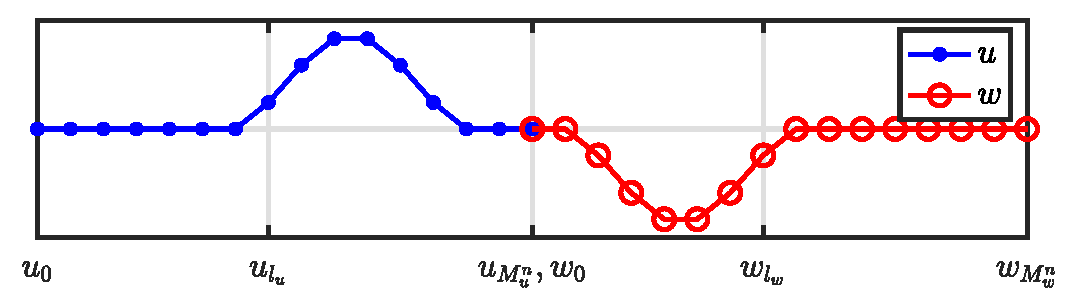
\includegraphics[width=\figwidth\columnwidth]{twoFreeStringsNarrow.eps}}}\\
    \vspace{-1em}\subfloat[]{\label{fig:twoFreeStringsGridMove}{ 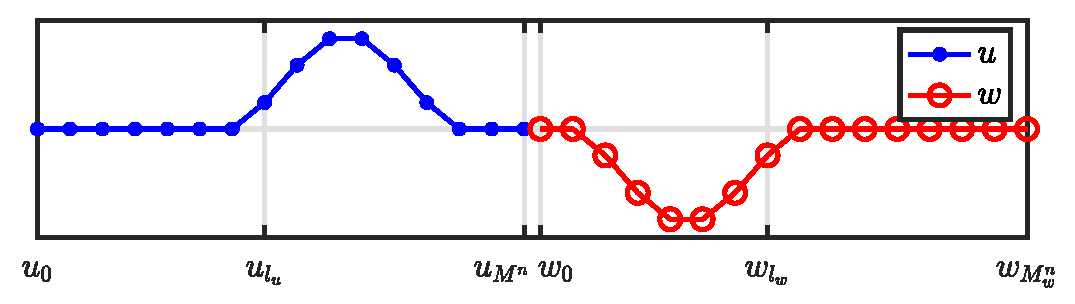
\includegraphics[width=\figwidth\columnwidth]{twoFreeStringsGridMoveNarrow.eps}}}\\
    \vspace{-1em}\subfloat[]{\label{fig:twoFreeStringsGridZoomed}{ 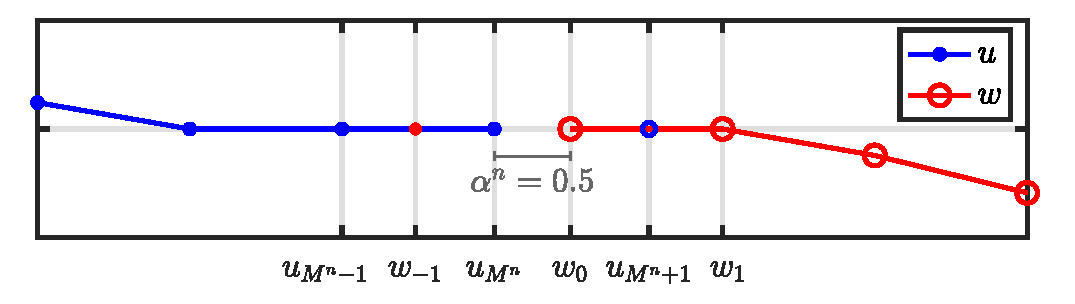
\includegraphics[width=\figwidth\columnwidth]{twoFreeStringGridMoveZoomedNarrow.eps}}}
    \vspace{-1em}\caption{Illustration of the dynamic grid. System $q_l^n$ in Eq. \eqref{eq:1dWaveDisc} is split into subsystems $v_\lv^n$ and $w_\lw^n$ (Eq. \eqref{eq:splitFDS}). The x-axis shows the location of the respective grid points with `$x^n$' omitted for brevity. 
    (a) $\Nfrac^n = 30$. As $\Nfrac^n = N^n$, the inner boundaries overlap. (b) $\Nfrac^n = 30.5$. The wave speed $c^n$ and thus $h^n$ are decreased, $\Nfrac^n \neq N^n$ and the inner boundaries no longer overlap. (c) Figure \ref{fig:twoFreeStringsGridMove} zoomed-in. All grid points (including virtual grid points) used in Eq. \eqref{eq:connectionInterpol} are shown. The distance between the inner boundaries is expressed using $\alpha^n$ in Eq. \eqref{eq:alphaDef}. (Image adapted from \cite{Willemsen2021a}.)}
\end{figure}

With reference to Eq. \eqref{eq:gridLocations}, the grid locations $\lv = 0$ and $\lw = \Mw$ are referred to as the \textit{outer boundaries} and are fixed to be at the limits of the system domain, i.e., $x_{v_0}^n = 0$ and $x_{w_{\Mw}}^n = L^n, \forall n$. Furthermore, Dirichlet boundary conditions are imposed on the outer boundaries according to Eq. \eqref{eq:discDirichlet}. 
The grid locations $\lv = \Mv$ and $\lw = 0$  are referred to as the \textit{inner boundaries}, at which Eq. \eqref{eq:splitFDS} (after expansion) requires a definition for the \textit{virtual grid points} $v_{\Mv+1}^n$ and $w_{-1}^n$. If $\Nfrac^n = N^n$, i.e. $\Nfrac^n$ is an integer, the inner boundaries overlap and the following condition must be satisfied:
\begin{equation}\label{eq:rigid}
    v_{\Mv}^n = w_0^n, \quad \text{if}\  x_{v_{\Mv}}^n =  x_{w_0}^n,
\end{equation}
This acts as a continuity constraint at the inner boundaries. As shown in
\cite{Willemsen2021a}, setting 
%combining this condition with Neumann boundary conditions \SBcomment[OK, here I guess we do need the Neumann conditions...still not clear to me why though. Like, is this condition in addition to the Dirichlet condition? This seems weird to me---you can't normally specify two conditions at an endpoint (think of the end of a string---you can't have both Dirichlet and Neumann satisfied, otherwise the solution is just zero)] \SWcomment[Alright, I plan to avoid the Neumann comment to avoid confusion, but just to clarify: the subsystems initially have Dirichlet outer boundaries and Neumann inner boundaries (so the system shown in Fig. \ref{fig:twoFreeStrings} is essentially ``free" in the center). When adding the rigid connection (which is not a boundary condition) to the inner boundaries when these are perfectly overlapping, the definition of the virtual grid points reduces to Eq. \eqref{eq:perfectOverlap} (see \cite{Willemsen2021a} (Sec. 4.1.1) for the derivation), and the system \eqref{eq:splitFDS} exhibits identical behaviour to the original system in Eq. \eqref{eq:1dWaveDisc}. This is purely used as a starting point! When the inner boundaries do not overlap, the Neumann + rigid connection does not hold, and we resort to the alternative definition for the virtual grid points in Eq. \eqref{eq:connectionInterpol}.] imposed on the inner boundaries shows that
the virtual grid points needed to calculate $v_{\Mv}^n$ and $w_0^n$ according to
\begin{equation}\label{eq:perfectOverlap}
    v_{\Mv+1}^n = w_1^n \qaq w_{-1}^n = v_{\Mv-1}^n,
\end{equation}
causes Eq. \eqref{eq:splitFDS} to exhibit identical behaviour to the original system in Eq. \eqref{eq:1dWaveDisc}.

Consider a decrease in wave speed $c^n$, which yields a decrease in $h^n$. This causes all grid points to move towards their respective outer boundary according to Eq. \eqref{eq:gridLocations} (see Figure \ref{fig:twoFreeStringsGridMove}). As the inner boundaries no longer overlap, i.e., $\Nfrac^n \neq N^n$, Eq. \eqref{eq:perfectOverlap} can no longer be used and alternative definitions for the virtual grid points need to be found. To this end, quadratic %\SBcomment[Quadratic: is this correct? Like it is a three-point interpolant? This is kind of odd, as normally you interpolate using an even number of points (so linear, cubic, etc. But it might be correct!)] \SWcomment[Yes, indeed! This is why it initially took so long to get nice behaviour for the modes, because I was only looking at odd-ordered interpolants. See \cite{Willemsen2021Thesis} (Sec. 12.3) for a comparison.] 
Lagrange interpolation can be used:
\begin{subequations}\label{eq:connectionInterpol}
    \begin{align}
            &v_{\Mv+1}^n = \Aterm v_{\Mv}^n + w_0^n - \Aterm w_1^n,
        \label{eq:calcUMP1}\\
            &w_{-1}^n = -\Aterm v_{\Mv-1}^n + v_{\Mv}^n+\Aterm w_{0}^n,\label{eq:calcWM1}
    \end{align}
\end{subequations}
where
\begin{equation}\label{eq:aterm}
    \Aterm = \frac{\alpha^n-1}{\alpha^n+1},
\end{equation}
and 
\begin{equation}\label{eq:alphaDef}
    \alpha^n = \Nfrac^n - N^n
\end{equation}
is the fractional part of $\Nfrac^n$. (Notice that $0\leq \alpha^n < 1$.) Also see Figure \ref{fig:twoFreeStringsGridZoomed}. For results of experiments with other interpolators, see \cite[Sec. 12.3]{Willemsen2021Thesis}.

\subsection{Matrix Form}\label{sec:matrixForm}
Similar to Sec. \ref{sec:matrixFormOrig}, one can define a general update equation of a system including the dynamic grid as
\begin{equation}\label{eq:generalDynGridMatrix}
    \AA \uStack^{n+1} = \BB \uStack^n + \CC \uStack^{n-1},
\end{equation}
where the definitions of $\AA$, $\BB$ and $\CC$ depend on the system at hand. %\SWcomment[Notice that the script style is used for the matrices and the state vector to indicate that this is a dynamic scheme.] 
Furthermore, $\MoneD \times 1$ vector
\begin{equation}\label{eq:uStack}
    \uStack^n = \begin{bmatrix}
    (\v^n)^T, (\w^n)^T
    \end{bmatrix}^T,
\end{equation}
% \SBcomment[Might possibly be better to choose a new letter (like v) for the combined vector, so as to avoid confusion with the earlier definition of u.] \SWcomment[I want to move towards a general definition that I can use for the 2D case as well. I also use $\v$ there for the building the stacked column vector in \eqref{eq:stacked2D}, but then again, there are a lot of overlaps with the symbols used in the 1D and 2D case. Hope that that's ok, and I don't have to come up with new ones.. haha. Could possibly add subscripts 1 and 2 to indicate whether it's 1D or 2D.] \SBcomment[Also: why are these vectors/matrices in script style? I mean, they're still just vectors and matrices, right?] \SWcomment[The script style was because it possibly better shows that these are related to a dynamic scheme rather than a static one (though I should probably elaborate on that for clarity).. Do script style symbols usually have a special meaning? ] \SBcomment[No, no special meaning, but it's extra notational baggage to carry around...]
with $\MoneD = \Mv + \Mw$, includes the state of the subsystems in Eq. \eqref{eq:splitFDS}. Here, $\v^n = [v_1^n, v_2^n, \hdots, v_{\Mv}^n]^T$ and $\w^n = [w_0^n, w_1^n, \hdots, w_{\Mw-1}^n]^T$ which are $\Mv \times 1$ and $\Mw \times 1$ respectively. 
The 1D wave equation including the dynamic grid can then be written in matrix form as Eq. \eqref{eq:generalDynGridMatrix} with
\begin{equation}\label{eq:1DwaveDynMatrix}
\begin{gathered}
    \AA = \I_{\MoneD}, \quad \BB = 2\I_\MoneD + (\lambda^n)^2\DDxx,\\
\text{and} \quad\CC = -\I_{\MoneD},
\end{gathered}
\end{equation}
% \begin{equation}\label{eq:1DwaveDynMatrix}
%     \uStack^{n+1} = \left(2\I_\MoneD + (\lambda^n)^2\DDxx\right)\uStack^n - \uStack^{n-1} 
% \end{equation}
where $\lambda^n = c^nk/h^n$ (which can always be set to 1 in the case of the 1D wave equation, yielding optimal simulation quality at all times), and $\DDxx$ is an adapted version of $\Dxx$ in Eq. \eqref{eq:dxxMat} to include the quadratic interpolation presented in Eq. \eqref{eq:connectionInterpol}:
\begin{equation}\label{eq:magicMatrix}
    \!\!\!\!\!\!\DDxx = \begin{bmatrix}[cccc|cccc]
     & \ddots  &\ddots & & & & \mathbf{0} & \\
       & \ddots & -2 & 1 & & & & \\
      & & 1 & \Aterm -2 & 1 & -\Aterm & \\ \cline{2-7}
      & & & & & & & \\[-0.9em]
      & & -\Aterm & 1 & \Aterm -2 & 1 & & \\[-0.5em]
         & & & &1 & -2 & \ddots  \\
         & \mathbf{0} & &  &  &\ddots & \ddots &
    \end{bmatrix}
\end{equation}
and is of size $\MoneD \times \MoneD$. In the extreme case that one of the systems only has one moving grid point, e.g., if $\w^n =[w_0^n]$, the lower-right quadrant in Eq. \eqref{eq:magicMatrix} will only have one entry (being $\Aterm-2$), and the lower-left and top-right quadrants will only have one row and one column respectively. 

\subsection{Adding and Removing Grid Points}\label{sec:addRemove}
If $c^n$ is decreased such that $N^n > N^{n-1}$, a grid point is added to the system. One can add points to either $\v$ or $\w$, or to both in an alternating fashion as in \cite{Willemsen2021a}, but here, only changes in $\v$ are considered. A grid point can be added to $\v$ using the following operations
\begin{equation}
\begin{aligned}
    \v^n &:= [(\v^n)^T, I_3^n\z^n]^T,\\
    \v^{n-1} &:= [(\v^{n-1})^T, I_3^n\z^{n-1}]^T,\\
\end{aligned} \quad \text{if } N^n > N^{n-1},
\end{equation}
%\SBcomment[OK, this is getting kind of hard to follow. In (24) above, you have $v^{n}$ defined in terms of $v^{n}$...like, are you resetting $v^{n}$?] \SWcomment[I see how this is confusing. I'm simply appending the state vector $\v^n$ with the new grid point. Maybe I should use $:=$, to indicate that it's more an operation rather than an equality?] \SBcomment[Also: I'm a little confused...before you were talking about quadratic interpolation, but now we're using cubic?] \SWcomment[Yes! For the state of the newly added grid point I use cubic interpolation.] 
where
\begin{equation*}
    \begin{aligned}
        \z^n &= [v_{M_v^{n-1}-1}^n, v_{M_v^{n-1}}^n, w_0^n, w_1^n]^T, \quad \text{and}\\
        \z^{n-1} &= [v_{M_v^{n-1}-1}^{n-1}, v_{M_v^{n-1}}^{n-1}, w_0^{n-1}, w_1^{n-1}]^T.
    \end{aligned}
\end{equation*}
Notice that $I_3^n$ is used for adding a grid point to both $\v^n$ and $\v^{n-1}$ and that $M_v^{n-1}$ is used as an index for both $v^n_\lv$ and $v^{n-1}_\lv$.
Furthermore, cubic Lagrangian interpolator
\begin{equation}\label{eq:customIp}
    I_3^n = \begin{bmatrix} -\frac{\alpha^n(\alpha^n+1)}{(\alpha^n+2)(\alpha^n+3)} &\frac{2\alpha^n}{\alpha^n+2} &\frac{2}{\alpha^n+2} 
    &-\frac{2\alpha^n}{(\alpha^n+3)(\alpha^n+2)}
    \end{bmatrix},
\end{equation}
where $\alpha^n$ is as defined in Eq. \eqref{eq:alphaDef}. Notice that, as $\alpha^n \gtrsim 0$ the moment a grid point is added (due to sub-audio rate parameter variations), $I_3^n\approx [0, 0, 1, 0]$ and the state of the added grid point is almost fully determined by the state of the inner boundary $w_0^n$. 

Removing grid points happens through simple deletion. If $c^n$ is increased such that $N^n < N^{n-1}$, a point is removed from $\v$ according to
\begin{equation}\label{eq:removePoint}
\begin{aligned}
    \v^n &:= [v_1^n, \hdots, v_{M_v^{n-1}-1}^n]^T,\\
    \v^{n-1} &:= [v_1^{n-1}, \hdots, v_{M_v^{n-1}-1}^{n-1}]^T,
    \end{aligned} \quad \text{if } N^n < N^{n-1}.
\end{equation}
It must be noted that for lossless systems, removing grid points could cause audible artefacts. This will be discussed in Sec. \ref{sec:removingGridPoints}. Furthermore, the limit on changing grid configurations is the addition / removal of one grid point per sample, but this limit needs to be much lower to retain the sub-audio rate assumption mentioned before. %In \cite{Willemsen2021b}, a lower limit of 20 samples per change is used together with $\lambda = 0.999$ and yields no noticeable artefacts.

% \subsection{State Correction}\label{sec:stateCorrection}
% At the moment that a point is removed, and thus $x_{v_{\Mv}}^n \approxeq x_{w_0}^n$, the states of the inner boundaries might not be approximately equal, i.e., $v_{\Mv}^n \not\approxeq w_0^n$. This violates the rigid connection in Eq. \eqref{eq:rigid} and -- in practice -- causes audible artefacts. To reduce this, a method of \textit{state correction}\footnote{\textit{displacement correction} in \cite{Willemsen2021a}.} is introduced and adds an artificial spring force between the inner boundaries:
% \begin{align*}
%     \dtt v_\lv^n = (c^n)^2\dxx v_\lv^n+ J_u(x_{v_{\Mv}}^n)
%     F_\text{c}^n,\\
%     \dtt w_\lw^n = (c^n)^2\dxx w_\lw^n - J_w(x_{w_0}^n)
%     F_\text{c}^n,
% \end{align*}
% where
% \begin{equation}\label{eq:spreadingOperators}
%     \begin{aligned}
%     J_u(x_i^n)& =
%     \begin{cases}
%         \frac{1}{h^n}, & \lv = \lfloor x_i^n/h^n\rfloor\\
%         0,& \text{otherwise}
%     \end{cases}
%     \quad\text{and}\\
%     J_w(x_i^n) &=
%     \begin{cases}
%         \frac{1}{h^n}, & \lw = \lfloor x_i^n/h^n \rfloor - \Mv\\
%         0,& \text{otherwise}
%     \end{cases}
% \end{aligned}
% \end{equation}
% apply the correction force to the inner boundaries. 
% Defining centred averaging and difference operators as
% \begin{subequations}\label{eq:centredOperators}
% \begin{align}\label{eq:centredAverage}
%     \mu_{t\cdot}q_l^n &= \frac{1}{2} \left(q_l^{n+1} + q_l^{n-1}\right),\\
%     \delta_{t\cdot}q_l^n &= \frac{1}{2k} \left(q_l^{n+1} - q_l^{n-1}\right),
% \end{align}
% \end{subequations}
% the effect of the artificial spring can be defined as
% \begin{equation}\label{eq:dispCorrForce}
%     F_\text{c}^n = \beta^n \left(\mu_{t\cdot}\eta^n +\sigma_\text{sc}\delta_{t\cdot}\eta^n \right),
% \end{equation}
% with damping coefficient $\sigma_\text{sc}$ and
% \begin{equation}\label{eq:betaDef}
%     \beta^n = \beta(\alpha^n) = \frac{1-\alpha^n}{\alpha^n}.
% \end{equation}
% Note that Eq. \eqref{eq:betaDef} is still defined for $\alpha^n = 0$ when solving for the connection force and acts as a rigid connection. See \cite[Ch. 12]{Willemsen2021Thesis} for a derivation. It is also important to note that despite the appearance of future grid values in Eq. \eqref{eq:centredOperators}, the correction force can be calculated explicitly. 

\section{DAMPED STIFF STRING}\label{sec:stiffString}
Using the matrix in Eq. \eqref{eq:magicMatrix} as a starting point, one can extend the dynamic grid method to more complex systems. A commonly used 1D model is the damped stiff string (see e.g. \cite{Willemsen2019}) which is described by the following partial differential equation (PDE) \cite{Bensa2003}:
\begin{equation}\label{eq:stiffString}
    \ptt q = c^2 \pxx q - \kappa^2 \pxxxx q - 2\sigma_0\pt q + 2\sigma_1\pt\pxx q,
\end{equation} 
with stiffness coefficient $\kappa$ (in m$^2$/s), and frequency-independent and frequency-dependent damping coefficients $\sigma_0$ (in s$^{-1}$) and $\sigma_1$ (in m$^2$/s).

Using
\begin{subequations}
\begin{align}
    \dtd \qln &= \frac{1}{2k}\left(q_l^{n+1} - q_l^{n-1}\right) \approxeq \pt q,\quad  \text{and}\\
     \dtm \qln &= \frac{1}{k}\left(\qln- q_l^{n-1}\right) \approxeq  \pt q,
\end{align}
\end{subequations}
Eq. \eqref{eq:stiffString} can be discretised using the following FDTD scheme:
\begin{equation}\label{eq:stiffStringFDS}
    \!\!\!\!\!\!\!\!\!\dtt \qln \!=\! c^2 \dxx \qln \!-\! \kappa^2 \dxxxx \qln\!\! -\! 2\sigma_0\dtd \qln\! +\! 2 \sigma_1 \dtm \dxx \qln,\!\!\!
\end{equation}
where $\dxxxx = \dxx\dxx$. The first-order temporal operators for the damping terms are chosen like this to keep the system explicit. Note that the stability condition is now $h\! \geq\! \sqrt{\tfrac{1}{2}\left(c^2k^2 + 4\sigma_1 k + \sqrt{(c^2k^2 + 4\sigma_1k)^2 +16\kappa^2k^2}\right)}$ (in the time-invariant case).
Equation \eqref{eq:stiffStringFDS} can be written in matrix form using Eq. \eqref{eq:generalMatrixUpdate} with 
\begin{equation}\label{eq:stiffStringMats}
\begin{aligned}
    \A &= (1 + \sigma_0k)\I_{N-1},\\ \B &= 2\I_{N-1} + \lambda^2 \Dxx - \mu^2 \Dxxxx + \frac{2\sigma_1k}{h^2}\Dxx, \  \text{and}\\
    \C &= -(1 - \sigma_0k)\I_{N-1} - \frac{2\sigma_1k}{h^2}\Dxx,
\end{aligned}
\end{equation}
% and writing this scheme in matrix form yields
% \begin{equation}\label{eq:stiffStringDynMatrix}
%     \q^{n+1} = \left(2\I_{N-1} + \lambda^2 \Dxx - \mu^2 \Dxxxx\right)\q^{n} - \q^{n-1},
% \end{equation}
where $\mu = \kappa k/h^2$, and (for simply supported boundary conditions)
\begin{equation}\label{eq:DxxxxMat}
    \Dxxxx = \Dxx\Dxx,
\end{equation}
with $\Dxx$ as defined in Eq. \eqref{eq:dxxMat}.

To apply the dynamic grid to the stiff string, the definition of $\Dxx$ in Eqs. \eqref{eq:stiffStringMats} and \eqref{eq:DxxxxMat} can simply be replaced by the $\DDxx$ from Eq. \eqref{eq:magicMatrix}. With reference to the general form in Eq. \eqref{eq:generalDynGridMatrix}, the following matrices can then be applied to the alternative vector $\uStack$ from Eq. \eqref{eq:uStack} to yield the dynamic stiff string:
\begin{equation}\label{eq:stiffStringDynMatrix}
\begin{aligned}
    \!\!\!\!\!\!\!\!\!\!\AA &= (1 + \sigma_0^nk)\I_{\MoneD},\\
    \!\!\!\!\!\!\!\!\!\!\BB &= 2\I_{\MoneD} + (\lambda^n)^2 \DDxx - (\mu^n)^2 \DDxxxx + \frac{2\sigma_1^nk}{(h^n)^2}\DDxx,\\
    \!\!\!\!\!\!\!\!\!\!\CC &= -(1 - \sigma_0^nk)\I_{\MoneD} - \frac{2\sigma_1^nk}{(h^n)^2}\DDxx,
\end{aligned}
\end{equation}
where $\mu^n = \kappa^n k/(h^n)^2$ and (for simply supported boundary conditions) 
\begin{equation}\label{eq:4thOrder1D}
    \DDxxxx = \DDxx\DDxx.
\end{equation}
Notice that $\kappa^n$, $\sigma_0^n$ and $\sigma_1^n$ are now allowed to be time-varying. Furthermore, $h^n$ can be obtained by calculating the stability condition with equality. %Also note that damping terms have been excluded for brevity, but can be added trivially.
Sound examples can be found via as well as an implementation of the dynamic stiff string can be found via \cite{soundExamples}. One example shows a string being made more inharmonic by increasing $\kappa^n$ but decreasing $c^n$ to retain the same pitch. Another varies $L^n$, $c^n$, $\kappa^n$, $\sz^n$ and $\so^n$ such that the timbral qualities of the string vary between a regular string, its octave, a vibraphone and a marimba.
\section{2D SYSTEMS}\label{sec:2D}
This section extends the framework presented in Sec. \ref{sec:dynamicGrid} to higher-dimensional systems. 

A rectangular 2D system can be described by a state variable $q = q(x,y,t)$ defined over $(x ,y) \in [0, L_x] \times [0, L_y]$ with sidelengths $L_x$ and $L_y$ (both in m). Discretising $q$ will result in grid function $q_{l,m}^n$ where $l \in \{0, \hdots, N_x\}$ and $m \in \{0, \hdots, N_y\}$, and the number of intervals in the $x$ and $y$-direction are $N_x = \floor[L_x/h]$ and $N_y = \floor[L_y/h]$ respectively. Notice that the same grid spacing $h$ is used in both the $x$ and $y$-direction, which is typical for isotropic, homogeneous systems.

Higher-dimensional systems can be written in matrix form by stacking or `flattening' the state. For Dirichlet or simply supported boundary conditions, the following $(N_x-1)(N_y-1)\times 1$ vector can be used to describe the state:
\begin{equation}\label{eq:stackedQ}
    \begin{aligned}
        \q^n &= [(\qq_{1}^n)^T, \hdots, (\qq_{N_x-1}^n)^T]^T \quad \text{with}\\
        \qq_l^n &= [q_{l, 1}^n, \hdots, q_{l, N_y-1}^n ]^T.
    \end{aligned}
\end{equation}
% The rest of this section starts by extending the dynamic grid to 2D after which it will be applied to the 2D wave equation and the thin plate. 

\subsection{2D Dynamic Grid}
Rather than splitting the original system into two subsystems, one can split it into four. Consider grid function $u_{i, l_i, m_i}^n$, where $i\in\{1, \hdots, 4\}$ is the index of the subsystem (also see Figure \ref{fig:2DGrid}). 
\begin{figure}[b]
    \centering
    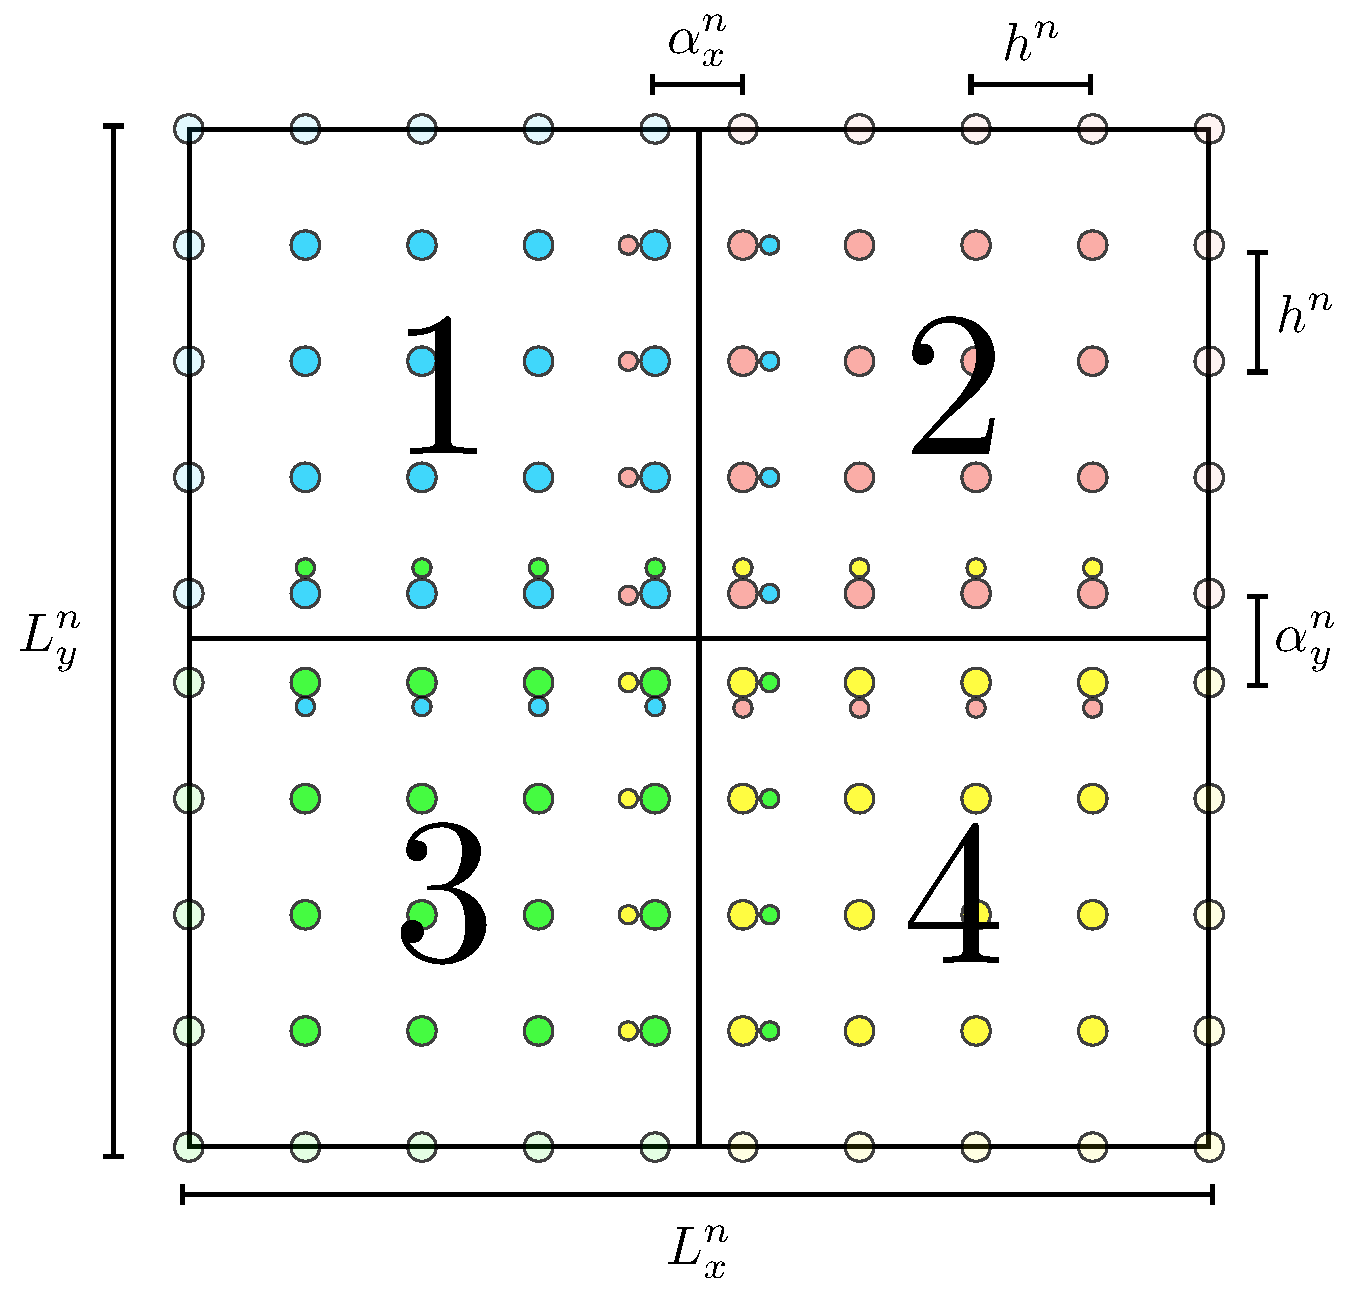
\includegraphics[width=\columnwidth]{2DDynamicGrid.pdf}
    \caption{Applying the dynamic grid to a 2D system. Virtual grid points are denoted as smaller circles and boundary points are not included in the calculation (for Dirichlet / simply supported boundary conditions). 
    %Indices along the $x$-direction increment from left to right, and those along the $y$-direction from top to bottom.
    }
    \label{fig:2DGrid}
\end{figure}
%
The subsystems are subdivided into $M_{x,i}^n$ intervals in the $x$-direction and $M_{y,i}^n$ intervals in the $y$-direction and the spatial indices have the following ranges: $l_i \in\{0, \hdots M_{x,i}^n\}$ and $m_i \in\{0, \hdots M_{y,i}^n\}$. 

Subsystems placed next to each other in the $x$-direction need to have the same number of points in the $y$-direction and vice versa. In other words, the following constraints apply to the number of intervals per subsystem:
\begin{equation*}
    M_{x, 1}^n = M_{x, 3}^n,\ \ M_{x, 2}^n = M_{x, 4}^n,\ \ M_{y, 1}^n = M_{y, 2}^n,\ \ M_{y, 3}^n = M_{y, 4}^n.
\end{equation*}
Furthermore, $0<M_{x,1}^n<N_x^n$ and $M_{x,2}^n = N_x^n-M_{x,1}^n$, and $0<M_{y,1}^n<N_y^n$ and $M_{y,3}^n = N_y^n-M_{y,1}^n$.

The grid points of each of the subsystems are positioned in the $x$-$y$-plane as follows:%, such that the systems in order are top-left, top-right, bottom-left, bottom-right:  
\begin{subequations}
    \begin{align}
        &\!\!\!\left(x_{u_{1, l_1, m_1}}^n, y_{u_{1, l_1, m_1}}^n\right) = \left(l_1h^n, m_1h^n\right),\\
        &\!\!\!\left(x_{u_{2, l_2, m_2}}^n, y_{u_{2, l_2, m_2}}^n\right) =  \left(L_x^n-(M_{x,2}^n-l_2)h^n, m_2h^n\right),\\
        &\!\!\!\left(x_{u_{3, l_3, m_3}}^n, y_{u_{3, l_3, m_3}}^n\right) = \left(l_3h^n, L_y^n-(M_{y,3}^n-m_3)h^n\right),\\
        &\!\!\!\begin{aligned}\left(x_{u_{4, l_4, m_4}}^n, y_{u_{4, l_4, m_4}}^n\right) =
        \Big(&L_x^n-(M_{x,4}^n-l_4)h^n,\\ \qquad &L_y^n-(M_{y,4}^n-m_4)h^n\Big).\end{aligned}
    \end{align}
\end{subequations}
Notice that, like in the 1D case in Eq. \eqref{eq:gridLocations}, the boundary points are fixed at the ends of the domain. If Dirichlet or simply supported boundary conditions are used, one can exclude the boundary points in the calculation and the ranges for the spatial indices become 
\begin{equation}\label{eq:rangesLM}
    \begin{aligned}
        l_1 &= \{1, M_{x,1}^n\}, &\quad m_1 &= \{1, M_{y,1}^n\}, \\
         l_2 &= \{0, M_{x,2}^n-1\}, &\quad m_2 &= \{1, M_{y,2}^n\},\\
        l_3 &= \{1, M_{x,3}^n\},&\quad m_3 &= \{0, M_{y,3}^n-1\},\\
        l_4 &= \{0, M_{x,4}^n-1\}, &\quad m_4 &= \{0, M_{y,4}^n-1\}.
    \end{aligned}
\end{equation}
Finally, one can define the inner boundaries that connect $u_1$ and $u_2$ as the first vertical inner boundary and those connecting $u_3$ and $u_4$ as the second vertical inner boundary. The same can be done for the first and second horizontal inner boundaries, which are those connecting $u_1$ and $u_3$, and $u_2$ and $u_4$, respectively. 

Similar to Eq. \eqref{eq:connectionInterpol} in the 1D case, virtual grid points at the first vertical and horizontal inner boundary are then calculated through
\begin{subequations}\label{eq:connectionInterpol2D}
    \begin{align}
            &\!\!\!\!\!\!\!\!u_{1, M_{x,1}^n+1, m_1}^n = \Aterm_x u_{1, M_{x,1}^n, m_1}^n + u_{2, 0, m_2}^n - \Aterm_x u_{2, 1, m_2}^n,\\
            &\!\!\!\!\!\!\!\!u_{2, -1, m_2}^n = -\Aterm_x u_{1, M_{x, 1}^n-1, m_1}^n\!\! + u_{1, M_{x,1}^n, m_1}^n\!\!+\Aterm_x u_{2, 0, m_2}^n,\\
            &\!\!\!\!\!\!\!\!u_{1, l_1, M_{y,1}^n+1}^n = \Aterm_y u_{1, l_1, M_{y,1}^n}^n + u_{3, l_3, 0}^n - \Aterm_y u_{3, l_3, 1}^n,\\
            &\!\!\!\!\!\!\!\!u_{3, l_3, -1}^n = -\Aterm_y u_{1, l_1, M_{y, 1}^n-1}^n + u_{1, l_1, M_{y,1}^n}^n+\Aterm_y u_{3, l_2, 0}^n,
    \end{align}
\end{subequations}
respectively, and can be applied in the same manner to the second vertical and horizontal inner boundaries. Here, similar to Eq. \eqref{eq:aterm} in the 1D case, 
\begin{equation}\label{eq:axayDef}
    \Aterm_x = \frac{\alpha_x^n-1}{\alpha_x^n+1}, \qaq \Aterm_y = \frac{\alpha_y^n-1}{\alpha_y^n+1},
\end{equation}
with 
\begin{equation}
    \alpha_x^n = \Nfrac_x^n - N_x^n, \qaq \alpha_y^n = \Nfrac_y^n - N_y^n,
\end{equation}
and fractional number of intervals in the $x$ and $y$-direction $\Nfrac_x^n = L_x^n / h^n$ and $\Nfrac_y^n = L_y^n / h^n$ respectively.

\subsubsection{Matrix Form}
Similar to Eq. \eqref{eq:stackedQ}, one can stack the total state of the system into a single column vector. The order in which the subsystems are stacked, in terms of `column of subsystem no. \#', is: 1, 3, ..., 1, 3, 2, 4, ..., 2, 4. If Dirichlet or simply supported boundary conditions are used, the total state can then be described as the following $\MtwoD \times 1$ column vector:
\begin{equation}\label{eq:stacked2D}
     \uStack^n = [(\vv^n)^T, (\ww^n)^T]^T,
\end{equation}
with $\MtwoD =(M_{x, 1}^n + M_{x, 2}^n) (M_{y, 1}^n + M_{y, 3}^n)$. Here,
\begin{equation}\label{eq:vw}
\begin{aligned}
    \vv^n &= [(\v_{1}^n)^T,\hdots, (\v_{M_{x,1}^n}^n)^T]^T, \qaq\\
    \ww^n &= [(\w_{0}^n)^T, \hdots, (\w_{M_{x, 2}^n-1}^n)^T]^T,
\end{aligned}
\end{equation}
contain the states of subsystems 1 and 3, and 2 and 4 respectively:
\begin{equation*}
     \v_{j_1^n}^n = [(\u_{1, j_1^n}^n)^T, (\u_{3, j_1^n}^n)^T]^T, \ \ \w_{j_2^n}^n = [(\u_{2, j_2^n}^n)^T, (\u_{4, j_2^n}^n)^T]^T,
\end{equation*}
with $j_1^n = \{1, \hdots, M_{x,1}^n\}$ and $j_2^n = \{0, \hdots, M_{x,2}^n-1\}$. Finally, 
\begin{equation}\label{eq:2DuDefs}
    \begin{aligned}
         \u_{1,l_1}^n &= [u_{1, l_1, 1}^n, \hdots, u_{1, l_1, M_{y, 1}^n}^n]^T,
         \\
         \u_{2,l_2}^n &= [u_{2, l_2, 1}^n, \hdots, u_{2, l_2, M_{y, 2}^n}^n]^T,\\
         \u_{3,l_3}^n &= [u_{3, l_3, 0}^n, \hdots, u_{3, l_3, M_{y, 3}^n-1}^n]^T,\quad \text{and}\\
         \u_{4,l_4}^n &= [u_{4, l_4, 0}^n, \hdots, u_{1, l_4, M_{y, 4}^n-1}^n]^T,
     \end{aligned}
\end{equation}
where the ranges for $l_i$ are specified in Eq. \eqref{eq:rangesLM}.
\subsubsection{Adding and Removing Grid Points}
Addition and removal of grid points happens in a similar fashion as described in Sec. \ref{sec:addRemove}, the difference being that an entire row or column of grid points affected rather than a single grid point.

Only considering alterations in the left subsystems, a column can be added by carrying out the following operations on $\vv$ in Eq. \eqref{eq:vw}
\begin{equation}
\begin{aligned}
   \vv^n &:= [(\vv^n)^T, \Z^n(I_3^n)^T]^T,\\
   \vv^{n-1} &:= [(\vv^{n-1})^T, \Z^{n-1}(I_3^n)^T]^T,
   \end{aligned} \quad \text{if } N_x^n > N_x^{n-1},
\end{equation}
where
\begin{align*}
\Z^n &= [(\v_{M_{x,1}^{n-1}-1}^n)^T, (\v_{M_{x,1}^{n-1}}^n)^T, (\w_{0}^n)^T, (\w_{1}^n)^T] \quad \text{and}\\
\Z^{n-1} &= [(\v_{M_{x,1}^{n-1}-1}^{n-1})^T, (\v_{M_{x,1}^{n-1}}^{n-1})^T, (\w_{0}^{n-1})^T, (\w_{1}^{n-1})^T]
\end{align*}
contain the states of the vertical inner boundaries and their first neighbours in the $x$-direction. 

Only considering alterations in the top subsystems, a row can be added by carrying out the following operations on $\u_1$ and $\u_2$ in Eq. \eqref{eq:2DuDefs} 
\begin{equation*}
    \begin{aligned}
        \u_{1,l_1}^n &:= [(\u_{1,l_1}^n)^T, I_3^n \z_{1, l_1}^n]^T,\\
        \u_{2,l_2}^n &:= [(\u_{2,l_2}^n)^T, I_3^n \z_{2, l_2}^n]^T,\\
        \u_{1,l_1}^{n-1} &:= [(\u_{1,l_1}^{n-1})^T, I_3^n \z_{1, l_1}^{n-1}]^T,\\
        \u_{2,l_2}^{n-1} &:= [(\u_{2,l_2}^{n-1})^T, I_3^n \z_{2, l_2}^{n-1}]^T,
    \end{aligned}\quad \text{if } N_y^n > N_y^{n-1},
\end{equation*}
% where the matrix containing the states of the horizontal inner boundaries and their neighbours is defined as
% \begin{equation*}
%     \Z^n = [\z_{1, 1}^n, \hdots, \z_{1, M_{x,1}^{n-1}}^n, \z_{2, 0}^n, \hdots, \z_{M_{x,2}^{n-1}-1}^n],
% \end{equation*}
where 
\begin{align*}
    \z_{1,l_1}^n &= [u_{1, l_1, M_{y,1}^{n-1}-1}^n, u_{1, l_1, M_{y,1}^{n-1}}^n, u_{3, l_1, 0}^n, u_{3, l_1, 1}^n]^T,\\
    \z_{2,l_2}^n &= [u_{2, l_2, M_{y,2}^{n-1}-1}^n, u_{2, l_2, M_{y,2}^{n-1}}^n, u_{4, l_2, 0}^n, u_{4, l_2, 1}^n]^T,\\
    \z_{1,l_1}^{n-1} &= [u_{1, l_1, M_{y,1}^{n-1}-1}^{n-1}, u_{1, l_1, M_{y,1}^{n-1}}^{n-1}, u_{3, l_1, 0}^{n-1}, u_{3, l_1, 1}^{n-1}]^T, \quad \text{and}\\
    \z_{2,l_2}^{n-1} &= [u_{2, l_2, M_{y,2}^{n-1}-1}^{n-1}, u_{2, l_2, M_{y,2}^{n-1}}^{n-1}, u_{4, l_2, 0}^{n-1}, u_{4, l_2, 1}^{n-1}]^T,
\end{align*}
contain the horizontal inner boundaries and their first neighbours in the $y$-direction (the ranges for $l_1$ and $l_2$ are given in Eq. \eqref{eq:rangesLM}).

Removing grid points also happens in a similar fashion to the 1D case. Removing a column from the system happens according to 
\begin{equation}
\begin{aligned}
    \!\!\!\!\vv^n &:= [(\v_1^n)^T, \hdots, (\v_{M_{x,1-1}^{n-1}}^n)^T]^T,\\
     \!\!\!\!\vv^{n-1} &:= [(\v_1^{n-1})^T, \hdots, (\v_{M_{x,1-1}^{n-1}}^{n-1})^T]^T,
    \end{aligned}
\ \ \text{if } N_x^n < N_x^{n-1},
\end{equation}
and removing a row from the system happens according to
\begin{equation}
    \begin{aligned}
        \u_{1,l_1}^n &:= [u_{1,l_1, 1}^n, \hdots, u_{1,l_1, M_{y,1}^{n-1}-1}^n]^T,\\
        \u_{2,l_2}^n &:= [u_{2,l_2, 1}^n,\hdots, u^n_{2,l_2, M_{y, 1}^{n-1}-1}]^T,\\
        \u_{1,l_1}^{n-1} &:= [u_{1,l_1, 1}^{n-1}, \hdots, u_{1,l_1, M_{y,1}^{n-1}-1}^{n-1}]^T,\\
        \u_{2,l_2}^{n-1} &:= [u_{2,l_2, 1}^{n-1},\hdots, u^{n-1}_{2,l_2, M_{y, 1}^{n-1}-1}]^T,
    \end{aligned}\quad \text{if } N_y^n < N_y^{n-1}.
\end{equation}
% \subsubsection{State correction}
% Like in the 1D case presented in Sec. \ref{sec:stateCorrection}, an artificial spring force can be added to the inner boundaries to prevent audible artefacts when removing grid points. If the state correction is applied to all grid points along the inner boundaries except for those at the intersection of the horizontal and vertical inner boundaries, (i.e., $u_{1, M_{x,1}^n, M_{y,1}^n}^n$, $u_{2, 0, M_{y,2}^n}^n$,$u_{3, M_{x,3}^n, 0}^n$ and $u_{4, 0, 0}^n$) the system can still be solved explicitly.

\subsection{2D Wave Equation}
The PDE of the 2D wave equation is defined as
\begin{equation}\label{eq:2DWavePDE}
    \ptt q = c^2 \Delta q,
\end{equation}
with wave speed $c$ (in m/s) and Laplacian $\Delta = \pxx + \pyy$. Equation \eqref{eq:2DWavePDE} can be discretised to the following FDTD scheme:
\begin{equation}\label{eq:2DWaveFDS}
    \dtt \qlmn = c^2 \dDelta \qlmn\ ,
\end{equation}
where $\dDelta = \dxx + \dyy$ is the discrete Laplacian, and 
\begin{subequations}
\begin{align}
    \dxx \qlmn &= \frac{1}{h^2}\left(q_{l+1,m}^n - 2 \qlmn + q_{l-1,m}^n\right)\approxeq \pxx q,\\
    \dyy \qlmn &= \frac{1}{h^2}\left(q_{l,m+1}^n - 2 \qlmn + q_{l,m-1}^n\right)\approxeq \pyy q.
\end{align}
\end{subequations}
Finally, the stability condition is $h \geq \sqrt{2}c k$.

\subsubsection{Matrix Form}
Again assuming Dirichlet boundary conditions, one can define scaled (by $h^2$) matrix forms of $\dxx$ and $\dyy$ similar to Eq. \eqref{eq:dxxMat}, i.e., $(N_x-1)\times(N_x-1)$ matrix $\Dxx$ and $(N_y-1)\times(N_y-1)$ matrix $\Dyy$. These can be used to obtain a matrix form of the discrete Laplacian by performing a Kronecker sum \cite{Horn1991, Hamilton2016}:
\begin{equation}\label{eq:kroneckerSum}
    \DDeltamat = \Dyy \oplus \Dxx,
\end{equation}
which is of size $(N_x-1)(N_y-1)\times (N_x-1)(N_y-1)$.
%
Using same-sized identity matrix $\I = \I_{(N_x-1)(N_y-1)}$, one can use the general matrix form in Eq. \eqref{eq:generalMatrixUpdate} with $\q^n$ as defined in Eq. \eqref{eq:stackedQ}, and define the matrices as follows:
\begin{equation}
    \A = \I, \quad \B = 2\I + \lambda^2 \DDeltamat, \qaq \C = -\I,
\end{equation}
where, as in the 1D case, $\lambda = c k /h$.
% and the stacked state vector in Eq. \eqref{eq:stackedQ}, the scheme in Eq. \eqref{eq:2DWaveFDS} can then be rewritten in matrix form as
% \begin{equation}
%     \qq^{n+1} = (2\I + \lambda^2\DDeltamat)\qq^n - \qq^{n-1}.
% \end{equation}

To apply the dynamic grid to the 2D wave equation, one can use the general matrix form in Eq. \eqref{eq:generalDynGridMatrix} with state vector $\uStack^n$ from Eq. \eqref{eq:stacked2D} and
\begin{equation}\label{eq:2DwaveDynMatrix}
% \begin{gathered}
    \!\!\!\!\!\!\!\!\!\AA = \I_\MtwoD, \ \ \BB = 2\I_\MtwoD + (\lambda^n)^2\DDDelta,\ \ \CC = -\I_\MtwoD.
% \end{gathered}
\end{equation}
Here,
% \begin{equation}\label{eq:2DwaveDynMatrix}
%     \uStack^{n+1} = \left(2\I_\MtwoD + (\lambda^n)^2\DDdelta\right)\uStack^n -\uStack^{n-1}
% \end{equation}
$\MtwoD \times \MtwoD$ matrix
\begin{equation}\label{eq:dynamicKronecker}
    \DDDelta = \DDyy \oplus \DDxx,
\end{equation}
where $\DDxx$ and $\DDyy$ include the effect of the interpolation at the inner boundaries presented in Eq. \eqref{eq:connectionInterpol2D}, and are as defined in Eq. \eqref{eq:magicMatrix} with $\Aterm_x$ and $\Aterm_y$ as defined in Eq. \eqref{eq:axayDef} respectively. Finally, $h^n = \sqrt{2}c^n k$.

\subsection{Damped Thin Plate}\label{sec:thinPlate}
Similar to the damped stiff string presented in Sec. \ref{sec:stiffString}, one can extend the dynamic grid method to other systems using higher-order spatial derivatives.
Consider the PDE of a damped thin plate \cite{Bilbao2009}
\begin{equation}\label{eq:thinPlatePDE}
    \ptt q = -\kappa^2\Delta\Delta q -2\sigma_0\pt q +2\sigma_1\pt\Delta q,
\end{equation}
where parameters are similarly defined to the damped stiff string in Eq. \eqref{eq:stiffString}. This can be discretised to 
\begin{equation}\label{eq:thinPlateFDS}
    \!\!\!\!\!\!\!\!\dtt\qlmn = -\kappa^2\delta_{\Delta\Delta}\qlmn-2\sigma_0\dtd \qlmn +2\sigma_1\dtm\dDelta \qlmn,
\end{equation}
where $\delta_{\Delta\Delta} = \delta_{\Delta}\delta_{\Delta},$ and $h \geq 2\sqrt{\kappa k}$. 
Using state vector $\q^n$ from Eq. \eqref{eq:stackedQ}, Eq. \eqref{eq:thinPlateFDS} can be rewritten using the general matrix form in Eq. \eqref{eq:generalMatrixUpdate} using
\begin{equation}\label{eq:thinPlateMats}
\begin{gathered}
    \A = (1+\sigma_0k)\I, \quad \B = 2\I - \mu^2 \DDeltaDelta + \frac{2\sigma_1k}{h^2}\DDeltamat,\\
    \text{and} \quad\C = -(1-\sigma_0k)\I - \frac{2\sigma_1k}{h^2}\DDeltamat.
    \end{gathered}
\end{equation}
% \begin{equation}
%     \q^{n+1} = \left(2\I - \mu^2 \DDeltaDelta\right)\q^n - \q^{n-1}
% \end{equation}
Here, $\I = \I_{(N_x-1)(N_y-1)}$, and for simply supported boundary conditions, same-sized matrix
\begin{equation}\label{eq:DDeltaDelta}
    \DDeltaDelta = \DDeltamat\DDeltamat,
\end{equation}
with $\DDeltamat$ as defined in Eq. \eqref{eq:kroneckerSum}.

Similar to before, the dynamic grid can be applied to this system by replacing the definitions of $\DDeltamat$ in Eqs. \eqref{eq:thinPlateMats} and \eqref{eq:DDeltaDelta} by $\DDDelta$ from Eq. \eqref{eq:dynamicKronecker}. Using $\uStack^n$ from Eq. \eqref{eq:stacked2D}, the dynamic thin plate can be written as the general form in Eq. \eqref{eq:generalDynGridMatrix} with
\begin{equation}\label{eq:thinPlateDynMatrix}
\begin{aligned}
    \AA &= (1+\sigma_0^nk)\I_\MtwoD, \\
    \BB &= 2\I_\MtwoD - (\mu^n)^2 \DDDeltaDelta + \frac{2\sigma_1^nk}{(h^n)^2}\DDDelta,\quad \text{and}\\
    \CC &= -(1-\sigma_0^nk)\I_\MtwoD - \frac{2\sigma_1^nk}{(h^n)^2}\DDDelta.
    \end{aligned}
\end{equation}
% \begin{equation}\label{eq:thinPlateDynMatrix}
%     \uStack^{n+1} = \left(2\I_\MtwoD - (\mu^n)^2 \DDDeltaDelta\right)\uStack^n - \uStack^{n-1},
% \end{equation}
where $h^n = 2\sqrt{\kappa^n k}$, and for simply supported boundary conditions 
\begin{equation}\label{eq:4thOrder2D}
    \DDDeltaDelta = \DDDelta\DDDelta,
\end{equation}
which is of size $\MtwoD \times \MtwoD$. Sound examples can be found via \cite{soundExamples}. One example shows a change in $\kappa^n$ (and $\so^n$) modelling an increase in plate thickness, where another shows changes in $L_y^n$. 

\section{RESULTS}\label{sec:analysis}
% To evaluate the dynamic grid several analyses have been carried out... 
In this section, results from the dynamic schemes are presented using a modal analysis, as well as the behaviour of the systems when excited.
% \subsection{Stability Analysis}
% % Notes:

% \SWcomment[I can numerically show that for all dynamic grid update equations (without damping) written in one-step form, the eigenvalues of matrix $\BB$ (see eq. \eqref{eq:modalAnalysis}) are located on the unit circle for all values of $\alpha^n$ (given that the stability condition is satisfied). However, I can't algebraically prove this. I do know that this shows stability, as well as the absence of damping effects of the dynamic grid method (right?). Should I mention this fact somewhere? Such as ``It can be shown that ... for all values of $\alpha^n$ ..." even though I did not actually do this]

% \SWcomment[
% What I do know is that the determinant of $\BB$ is 1, for any value of $\alpha^n$ (but I suppose that counts for all matrices in 1-step form). Either way, I hope that that helps to prove something...]

\subsection{Modal Analysis}
One can retrieve the modal frequencies of the implementation of the dynamic grid by performing a modal analysis of the update equation in matrix form. For reference, the general form is Eq. \eqref{eq:generalDynGridMatrix} with matrices of the various systems defined in Eqs. \eqref{eq:1DwaveDynMatrix}, \eqref{eq:stiffStringDynMatrix}, \eqref{eq:2DwaveDynMatrix} and \eqref{eq:thinPlateDynMatrix}. Assuming $\sigma_0^n = \sigma_1^n = 0$, (as the influence of losses on modal frequencies are very small for damped systems), and for sub-audio rate parameter variations, the $p$\th numerical modal frequency can be calculated as
\begin{equation}\label{eq:modalAnalysis}
    f_p^n \approxeq \frac{1}{2 \pi k}\cos^{-1}\left(\frac{1}{2}\text{eig}_p(\BB)\right),
\end{equation}
where $\text{eig}_p(\cdot)$ denotes the ``$p$\th eigenvalue of."

To determine the accuracy of the frequencies obtained in Eq. \eqref{eq:modalAnalysis}, one can compare against modal frequencies against expected values.
% \SWcomment[not sure if I want to include the following, but just so you know how I did the analysis :) $\rightarrow$]
% The expected modal frequencies of a FDTD scheme as a function of the wave number can be obtained by performing a von Neumann analysis on the discrete scheme. The wave number as a function of physical parameters can then be obtained through a combination of dispersion analysis and modal analysis of the continuous PDE. \SWcomment[$\leftarrow$]
%
Results of a modal analysis of the dynamic stiff string with $\kappa^n \approx 1.26$ m$^2$/s and linear changes in $c^n$ corresponding to $\Nfrac^n = 15 \rightarrow 20$ can be seen in Fig. \ref{fig:resultsStiffString}, as well as the expected modal frequencies. 
%% other wording
% One can analyse the continuous-time equations and the FD scheme to retrieve the modal frequencies as a function of physical parameters. These will be the expected modal frequencies.
%
% These can be compared modal frequencies exhibited by the eventual implementation by performing a modal analysis on the update equation in matrix form including the dynamic grid. 
%
% \begin{figure}[t]
%     \centering
%     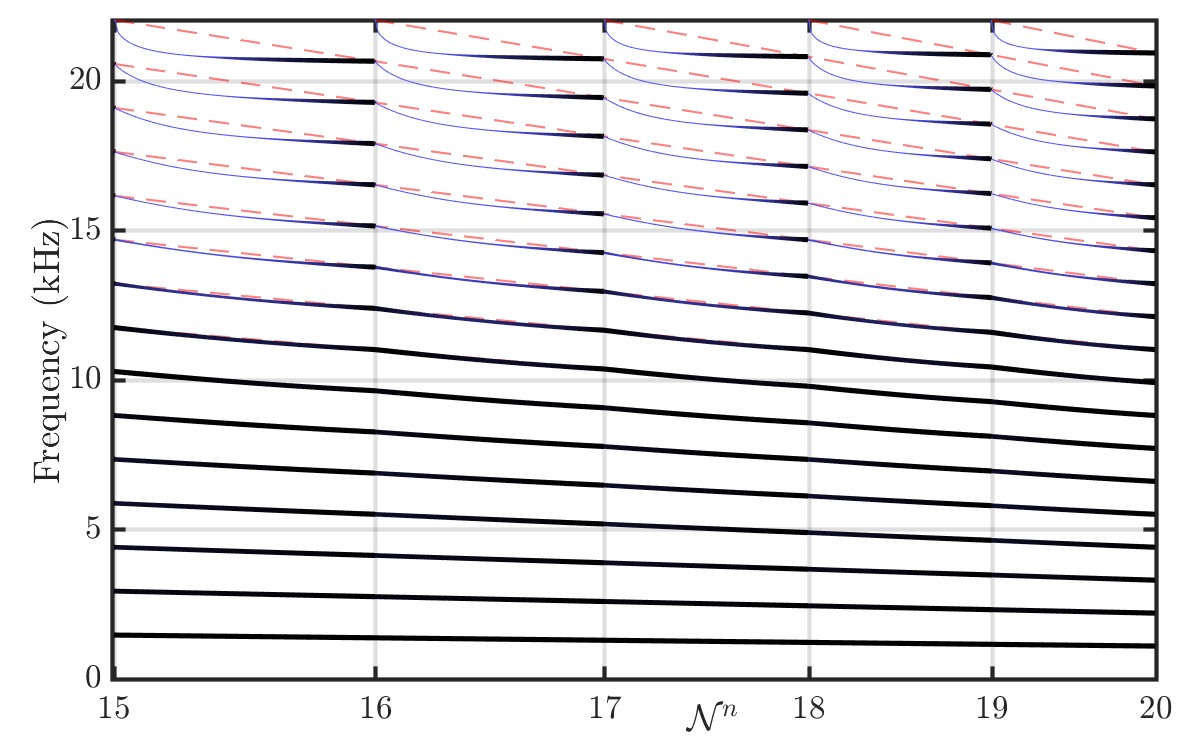
\includegraphics[width=\columnwidth]{stiffStringModes.eps}
%     \caption{Modal frequencies of the stiff string in Eq. \eqref{eq:stiffStringDynMatrix} with $\kappa \approx 1.26$ and (linear) changes in $c$ corresponding to $\Nfrac = 15 \rightarrow 20$. Modes exhibited by the system are shown in solid black, and expected modal frequencies are shown using dashed red lines.}
%     \label{fig:resultsStiffString}
% \end{figure}
\begin{figure}[t]
    \centering
    \subfloat[]{\label{fig:resultsStiffString}{ \includegraphics[width=\figwidth\columnwidth]{stiffStringModesNarrow.eps}}}\\
    \vspace{-1em}\subfloat[]{\label{fig:outputStiffSTring}{ 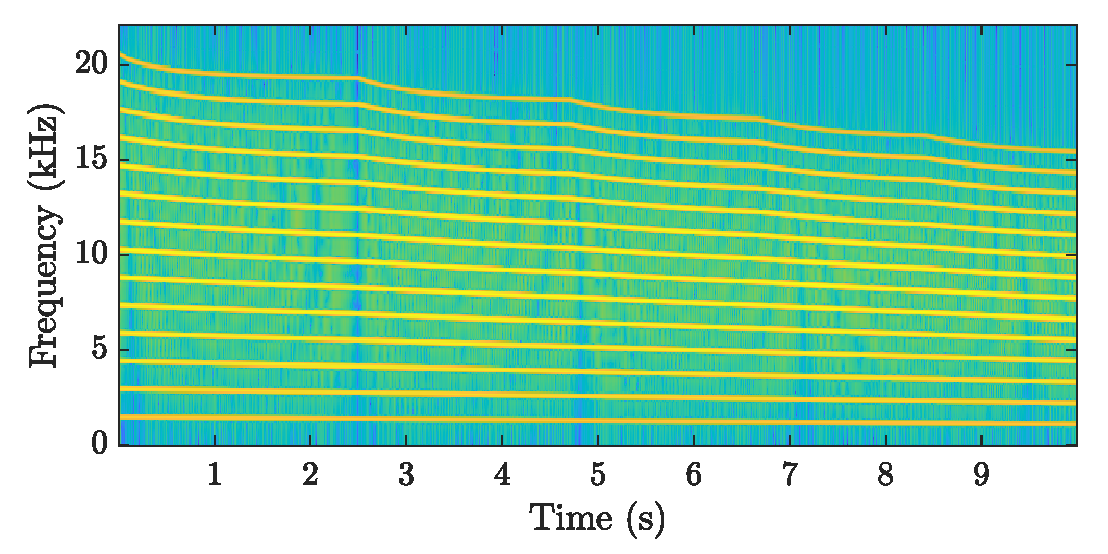
\includegraphics[width=\figwidth\columnwidth]{stiffStringOutput.eps}}}\\
    \vspace{-1em}\caption{The dynamic stiff string (Eq. \eqref{eq:generalDynGridMatrix} with Eq. \eqref{eq:stiffStringDynMatrix}) with $\kappa \approx 1.26$ and $c^n$ is (linearly) swept such that $\Nfrac^n = 15 \rightarrow 20$. (a) Results of Eq. \eqref{eq:modalAnalysis}. Modes exhibited by the system are shown in solid black, and expected modal frequencies are shown using dashed red lines. (b) Output of the dynamic stiff string excited at $n=0$ and $l=1$ and output retrieved at the same location ($\fs = 44.1$ kHz).}
\end{figure}
% One can retrieve the modal frequencies of a FD scheme by performing a modal analysis on its update equation in matrix form. These can be compared to the expected modal frequencies one can obtain from the continuous 
%
% \begin{table}[t]
% \tabcolsep8.1pt
% \caption{Tables should have a brief caption. Highlighting the best result(s) is helpful to readers.}
% \label{table:an_example_table}
% {%
% \begin{tabular}{@{}lllc@{}}\toprule
%  & \multicolumn{3}{c}{$\Nfrac$}\\\colrule
%  Model & 15 - 16 & 20 - 21 & 50 - 51  \\\hline
% 1D wave & -67.02 & -54.19 & -25.85 \\
%         Bar & -96.00 & -77.38 & -36.71\botrule
% \end{tabular}}
% \begin{tabnote}
% Note. This table contains several acronyms which should be defined in the paper, when they are first used (but not in the abstract).
% \end{tabnote}
% \end{table}
%
% In the following, the difference between the expected modal frequencies and those exhibited by the implementation will be expressed in cents.
%
The largeest frequency deviation for the dynamic stiff string with $N^n = 15$ is around $-67$ cents, whereas this decreases to around $-56$ cents for $N^n = 19$. This is similar to the results presented in \cite{Willemsen2021a}. Setting $c^n=0$ (effectively reducing the stiff string to an ideal bar \cite{Bilbao2009}), the maximum frequency deviation for $N^n=15$ is around -96 cents. 

Results for the dynamic thin plate appear in Table \ref{tab:2dresults}. It can be shown that for a square 2D system, the maximum frequency deviations are identical to the case of the analogous 1D system. In other words, the 1D wave equation and the 2D wave equation share maximum frequency deviations for equal values of $N^n$ (1D) and $N_x^n$ and $N_y^n$ (2D). This also holds for the ideal bar and the thin plate. This indicates that frequency deviations do not worsen when applying the dynamic grid to higher dimensional systems.% \SWcomment[(using the Kronecker sum in Eq. \eqref{eq:dynamicKronecker})].

In both the 1D and 2D cases, the system exhibits following behaviours:
\vspace{-1em}\begin{itemize}
    \item If $\alpha^n$ = 0 and parameters are static, the split system exhibits identical behaviour to the original. 
    \item The number of modes is always equal to the number of grid points in the system (excluding boundary points).
    \item The higher the mode number, the more its frequency deviates from the expected frequency for one value of $N^n$.
    \item The higher the total number of grid points in the simulation, the smaller the frequency deviation.
    \item The location where a system is split (and thus the location where grid points are added / removed) does not influence the frequency content. 
    % \item The highest deviation amount for one value of $N^n$ happens for $\alpha^n \lesssim 0.25$.
\end{itemize}
\vspace{-1em}
% \begin{table}[h]
%     \centering
%         \caption{Caption}

%     \begin{tabular}{|c|c|c|c|c|}
%         \hline & 15 - 16 & 20 - 21 & 50 - 51  \\\hline
%         1D wave & -67.02 & -54.19 & -25.85 \\
%         Bar & -96.00 & -77.38 & -36.71\\\hline
%     \end{tabular}
%     \label{tab:my_label}
% \end{table}

% \begin{table}[h]
%     \centering\fontsize{8pt}{9pt}\selectfont
%         \caption{Maximum frequency deviation for the dynamic thin plate (in cents), for different values of $\Nfrac_x$ and $\Nfrac_y$.}

%     \begin{tabular}{|c|c|c|c|c|c|}
%         \hline\backslashbox{$\Nfrac_x$}{$\Nfrac_y$} & 5-6 & 6-7 & 7-8 & 8-9 & 9-10 \\\hline
%         5-6 & -194.59 & -185.20 & -177.73 & -171.70 & -166.76\\\hline
%         6-7 & -185.20 &-175.69& -168.07 & -161.89 & -156.81\\\hline
%         7-8 & -177.73 & -168.07 &  -160.32 & -154.00 & -148.79\\\hline
%         8-9 & -171.70 & -161.89 & -154.00 & -147.56 & -142.24\\\hline
%         9-10 & -166.76 & -156.81 & -148.79 & -142.24 &-136.80\\\hline
%     \end{tabular}
%     \label{tab:2dresults}
% \end{table}

\begin{table}[h]
    \centering\fontsize{8pt}{9pt}\selectfont
        \caption{Maximum frequency deviation for the dynamic thin plate (in cents), for different values of $\Nfrac_x^n$ and $\Nfrac_y^n$.}

    \begin{tabular}{|c|c|c|c|c|c|}
        \hline\backslashbox{$\Nfrac_x^n$}{$\Nfrac_y^n$} & $15\!\!\rightarrow \!\! 16$ & $16\!\!\rightarrow \!\!17$ & $17\!\!\rightarrow \!\!18$ & $18\!\!\rightarrow \!\!19$ & $19\!\!\rightarrow \!\!20$ \\\hline
        $15\!\!\rightarrow \!\!16$ & -96.00 & -93.78 & -91.82 & -90.06 & -88.49 \\\hline
        $16\!\!\rightarrow \!\!17$ & -93.78 &-91.54  &-89.55 & -87.75 & -86.15 \\\hline
        $17\!\!\rightarrow \!\!18$ & -91.82 & -89.55 &  -87.52 &-85.69 &  -84.05 \\\hline
        $18\!\!\rightarrow \!\!19$ & -90.06 &  -87.75 & -85.69 &-83.84 & -82.16 \\\hline
        $19\!\!\rightarrow \!\!20$ & -88.49 &  -86.15 &  -84.05 & -82.16 & -80.47\\\hline
    \end{tabular}
    \label{tab:2dresults}
\end{table}
\vspace{-1em}
\subsection{System Behaviour}\label{sec:removingGridPoints}
Fig. \ref{fig:outputStiffSTring} shows the output of the dynamic stiff string (simulated at $\fs = 44.1$ kHz) with $\Nfrac^n = 15$ excited at $t=0$ s, after which $c^n$ is (linearly) swept such that $\Nfrac^n = 20$ at $t=10$ s. One can observe that the highest mode predicted by the analysis in Fig. \ref{fig:resultsStiffString} is not excited, which will be elaborated on in Sec. \ref{sec:discussion}. Furthermore, when a change in grid configuration occurs, the energy of modes follows the `path of least resistance' predicted in Fig. \ref{fig:resultsStiffString}. If modes of two grid configurations align, the energy transfer happens smoothly and no noticeable artefacts occur (under sub-audio rate parameter variations). This also means that every time a grid point, and thus a mode, is added at the top of the spectrum, it will not obtain any energy. If the system is excited at a later time, these modes will naturally be excited too.
% Furthermore, no noticeable artefacts occur when adding grid points (at sub-audio rate parameter variations). 

If, on the other hand, $\Nfrac^n = 20\rightarrow 15$ (effectively horizontally flipping Fig. \ref{fig:resultsStiffString}), modes seem to `disappear' around the Nyquist frequency when grid points are removed. As there are no modes in the new grid configuration to receive energy, its energy is distributed over the remaining modes, causing audible artefacts. Informal experiments show that if modes are damped before they `disappear', noticeable artefacts are prevented. In the case of the stiff string, this is what frequency-dependent losses automatically allow for. %If parameters are changed such that grid points are removed, noticeable artefacts are prevented for a high enough value $\sigma_1$. 
The minimum value required for $\sigma_1^n$ to damp the highest mode depends on various factors, such as the values of other parameters and the speed of parameter variation.
In the case of 2D systems, if parameters are varied such that grid points need to be removed, multiple grid points, and thus modes, `disappear' at once. Although these do not only include the highest frequency modes, damping does seem to take care of noticeable artefacts. 

For the lossless systems presented in this paper, local losses could be added at the inner boundaries, presented in \cite{Willemsen2021a, Willemsen2021b} as displacement / state correction. Although this successfully prevents noticeable artefacts, this method does introduce unnatural losses to the system.

% \SWcomment[One can also see it in time-space domain.] Consider the dynamic 1D wave equation in Eq. \eqref{eq:splitFDS} where $c$ -- and thus $h$ through Eq. \eqref{eq:gridLocations} -- is increased. The moment that a grid point is removed (according to Eq. \eqref{eq:removePoint}), and thus $x_{v_{\Mv}}^n \approxeq x_{w_0}^n$, the states of the inner boundaries might not be approximately equal, i.e., $v_{\Mv}^n \not\approxeq w_0^n$. This violates the rigid connection in Eq. \eqref{eq:rigid} and -- in practice -- causes audible artefacts. This fact also applies to the other (including 2D) systems presented in this paper. In \cite{Willemsen2021a}, we propose a method of \textit{displacement correction} that adds an artificial spring force to the inner boundaries, locally adding loss and successfully preventing (visible) artefacts. Although negligibly influencing the frequency content, this correction does introduce unnatural losses to the system. Frequency dependent damping decreases large differences between the inner boundaries...
\section{DISCUSSION}\label{sec:discussion}
As shown in Sec. \ref{sec:analysis}, modal frequencies exhibited by the dynamic grid deviate from those expected. However, the largest frequency deviations occur at higher-frequency ranges, which are less perceptually relevant, and will be ultimately experience high damping due to viscothermal effects. For the 1D systems presented in this paper, where a (quasi-)harmonic output is expected, these deviations could still cause beating effects, though listening tests will have to confirm this.

The fact that the highest mode predicted by the analysis in Fig. \ref{fig:resultsStiffString} is not excited as shown in Fig. \ref{fig:outputStiffSTring} can be explained by the fact that if $\alpha^n = 0$, two grid points are perfectly overlapping and will act as one grid point due to the rigid connection in Eq. \eqref{eq:rigid}. 

It is obviously not ideal to rely on (frequency-dependent) losses for grid points to be removed without noticeable artefacts. However, it can be argued that relying on losses which are often used in existing models is more natural than adding artificial damping at specific locations in the grid, such as done in previous work \cite{Willemsen2021a, Willemsen2021b}. %Furthermore, high-frequency losses occur naturally in any physical material. 

% If a grid point, and thus a mode is removed from the system, its energy will not be. All other modes will gain energy from the removed mode, which results in audible artefacts. In the 1D case, as the highest-frequency mode is the one that gets removed, the frequency-dependent damping takes care of this. \SWcomment[In the 2D case, the modes that are removed are not necessarily the highest frequency, and might not be damped before a row/column is removed.] Listening tests will have to confirm the absence of artefacts.


% The thin plate can be easily extended to the stiff membrane, which combines the 2D wave equation with the thin plate.

To implement FDTD schemes in matrix form in real-time using e.g. C++, they need to be rewritten to update equations. The updates at the inner boundaries for the 1D and 2D wave equations can be directly implemented using the definitions in Eqs. \eqref{eq:connectionInterpol} and \eqref{eq:connectionInterpol2D} respectively. For the schemes including a 4\textsuperscript{th}-order spatial derivative, one can retrieve the coefficients by performing the matrix multiplications presented in Eqs. \eqref{eq:4thOrder1D} and \eqref{eq:4thOrder2D} for the stiff string and thin plate respectively. 

% Notes:

% Multiplying the average slope of the line that connects the (higher-frequency) minima of each deviation in Hz by the values of $\Nfrac^n$ that causes these minima, yields lines that are bounded by the samplerate...

\section{CONCLUSION}\label{sec:conclusion}
This paper presents the dynamic grid, a method to smoothly change grid configurations of FDTD schemes allowing for runtime parameter variation. Furthermore, the CFL-type conditions of these schemes can be satisfied with equality at all times, maximising simulation quality or bandwidth for any choice of parameters. We extend previous work on the time-varying 1D wave equation in \cite{Willemsen2021a} by applying the dynamic grid to the stiff string, the 2D wave equation and the thin plate. 
% using FDTD schemes in matrix form and includi
% By writing a FDTD scheme in matrix form and including the effect of the dynamic grid there, we have been able to extend previous work one can use matrix operations to build higher-order and higher-dimensional systems.
%
Physical accuracy and stability conditions are not the main focus of this contribution, but rather the efficiency and applicability to already existing models.

Future directions include the extension of the method presented here to 3D, performing another Kronecker sum as in Eq. \eqref{eq:dynamicKronecker} for the 3\textsuperscript{rd} dimension (see \cite{Hamilton2016}). Other future considerations include listening tests to confirm the absence of audible artefacts, as well as real-time implementation and control, such that a player can `mold' their instrument while performing, potentially discovering new ways of expression.

\section{ACKNOWLEDGMENTS}
This  work  has  been  funded  in  part  by  the European Art-Science-Technology Network for Digital Creativity (EASTN-DC), project number 883023 and the Nordic Sound and Music Computing Network by Nordforsk. This work is also funded in part by the European Research Council (ERC) under the European Union’s Horizon 2020 research and innovation programme, Grant agreement No. 950084-StG-NEMUS. Thanks to the DAFx20in21 committee for providing the open access publication of this work.

\bibliography{jaes.bib}
\bibliographystyle{jaes.bst}

% \appendix
% \section*{APPENDIX: KRONECKER SUM}\label{app:kronecker}
% To obtain the matrix form of the discrete Laplacian in Eq. \eqref{eq:kroneckerSum} the Kronecker product and Kronecker sum need to be introduced. The Kronecker product between two matrices is \cite{Horn1991} 
% \begin{equation}
%     \A_{M\times N} \otimes \B_{K\times L} = \begin{bmatrix}
%         a_{11}\B & \hdots & a_{1N}\B\\
%         \vdots & \ddots & \vdots\\
%         a_{M1}\B & \hdots & a_{MN}\B\\
%     \end{bmatrix}_{MK \times NL},
% \end{equation}
% and the kronecker sum between two square matrices is \cite{Hamilton2016}
% \begin{equation}\label{eq:kronSum}
%     \A_{M \times M} \oplus \B_{N \times N} = \I_N\otimes \A + \B \otimes\I_M.
% \end{equation}

%Biography
 \biography{Silvin Willemsen}{JAESheadshotSilvin.jpg}{Silvin Willemsen is a Postdoctoral Researcher at Aalborg University in Copenhagen, Denmark. He received his MSc. in Sound and Music Computing from Aalborg University in 2017. In 2018, he was appointed as a PhD Stipend at the Department of Architecture, Design and Media Technology at Aalborg University Copenhagen and was affiliated with the Multisensory Experience Lab. In 2021 he received his PhD degree %entitled ``The Emulated Ensemble: Real-Time Simulation of Musical Instruments using Finite-Difference Time-Domain Methods'', 
 and continues to work in the field of physical modelling for musical instruments.}
 \biography{Stefan Bilbao}{stefan.jpg}{Stefan Bilbao (B.A. Physics, Harvard, 1992, MSc., PhD Electrical Engineering, Stanford, 1996 and 2001 respectively) is currently Professor of Acoustics and Audio Signal Processing in the Acoustics and Audio Group at the University of Edinburgh, and previously held positions at the Sonic Arts Research Centre, at the Queen's University Belfast, and the Stanford Space Telecommunications and Radioscience Laboratory. He is an Associate Editor of the IEEE/ACM Transactions on Audio Speech and Language Processing. He was born in Montreal, Quebec, Canada. }
 \biography{Michele Ducceschi}{ducceschi.jpeg}{Michele Ducceschi (BSc. Physics (2008), University of Padova, Italy, MSc. Acoustics (2010), University of Edinburgh, UK, PhD Mechanical Engineering (2014), ENSTA and Ecole Polytechnique, France) is an Associate Professor at the University of Bologna in Italy. He is currently the P.I. of the ERC-funded project NEMUS (2021-2026). Previously, he held positions at the University of Edinburgh. He was a Royal Society Newton International Fellow, and a Leverhulme Early Career Fellow.}
 \biography{Stefania Serafin}{Stefania.jpg}{Stefania Serafin is Professor of Sonic interaction design at Aalborg University in Copenhagen and the leader of the Multisensory Experience Lab together with Rolf Nordahl.
She is the President of the Sound and Music Computing (SMC) association, Project Leader of the Nordic SMC network and lead of the SMC Master at Aalborg University.
Stefania received her PhD % entitled “The sound of friction: computer models, playability and musical applications” 
from Stanford University in 2004. %, supervised by Professor Julius Smith III.
Her research on sonic interaction design, sound for virtual and augmented reality with applications in health and culture can be found \href{https://tinyurl.com/35wjk3jn}{here}.
}
\end{document}
